\section{}
	\textbf{Метрические пространства, нормированные пространства, евклидовы пространства. Примеры: $R_n,\ C[a, b]$, дискретная метрика, $l^{\infty}(S), l^1, l^2$, $p$-адическая метрика на $Q$, метрика Хаусдорфа (в неочевидных случаях неравенство треугольника можно не доказывать). Открытые множества в метрическом пространстве, их свойства. Открытость открытого шара.}\\
	\\
	\textbf{Определение}: Пусть X - множество, метрикой на Х называется отображение $\phi: X \times X \rightarrow \left[0,+ \infty\right)\subset\mathbb{R} (x,y)\rightarrow (x,y)$\\
	Причем:
	\begin{enumerate}
		\item $p(x,x) = 0\ \forall x \in X$
		\item $p(x,y) = p(y,x)\ \forall x,y \in X$
		\item $p(x,z)\leqslant p(x,y) + p(y,z)\ \forall x,y,z \in X$
		\item $p(x,y)>0\ \forall x\neq y$
	\end{enumerate}
	
	$(X,p)$ -- метрическое пространство. Если выполнены только условия (1) - (3), то полуметрическое пространство (и полуметрика соответственно)\\
	Примеры:
	\begin{enumerate}
		\item
		X--любое множество 
		$p(x,y)=
		\begin{cases}
		1\ \text{если}\ x\neq y\\
		0\ \text{если}\ x = y\\
		\end{cases}$
		
		\item
		$\mathbb{R}\ p(x,y) = |x - y|$
		
		\item
		метрики на $\mathbb{R}^{n}$:\\
		$p_1 (x,y) = \sum_{i = 1}^n |x_i- y_i|$\\
		$p_n (x,y) = \sqrt{\sum_{i = 1}^n (x_i^n-y_i^n)}$\\
		$p_\infty (x,y) = \max|x_i-y_i|$
		
		\item
		Равномерная метрика на $C[a,b]\ p(f,g) = \sup|f(t)-g(t)|, t\in [a,b]$\\
		В примерах было векторное пространство.	
	\end{enumerate}
	\textbf{Норма}\\
	Определние: Пусть Х ВП над полем $\mathbb{K} = \mathbb{C}\ \text{или}\ \mathbb{R}$\\
	Норма (Длина) на Х-отображение ||.|| : Х $\rightarrow [0;+ \infty)$
	\begin{enumerate}
		\item $||\alpha x||=|\alpha|\cdot ||x||$
		\item $||x + y|| \leqslant ||x||+||y||$
		\item $||x||>0$
	\end{enumerate}
	$(X, ||.||)$-нормированное простраство.
	Если выполнены только (1) и (2), то полунормированное пространство (полунорма).\\
	Наблюдение: $p(x,y) = ||x - y|| \Rightarrow $ Поэтому каждое нормированное пространство и его подмножества-метрические пространства.\\
	Примеры:
	\begin{enumerate}
		\item 
		Нормы на $\mathbb{K}^n$
		\begin{enumerate}
			\item ${||x||}_1 = \sum_{i = 1}^n |x_i|$
			\item ${||x||}_2 = \sqrt{\sum_{i = 1}^n |x_i^2|}$
			\item ${||x||}_n = \Bigg(\sum_{i = 1}^n |x_i^n|\Bigg)^{\frac{1}{n}}$
			\item ${||x||}_{\infty} = \max{|x_i|}$
		\end{enumerate}
		
		\item 
		Равномерная норма на $C[a,b]:\ ||f|| = \sup{f(t)}$, где $t \in [a,b]$\\
		\\
		Пусть Е-ВП над $\mathbb{R}$. скалярное произведение на Е-отображение $(x,y) \in E\times E\ \rightarrow \langle{x,y}\rangle \in \mathbb{R}$ \\
		Причем:
		\begin{enumerate}
			\item $\langle{\alpha x+ \beta y,z}\rangle=\alpha \langle{x,z} \rangle+\beta \langle{y,z}$
			\item $\langle{x,y} \rangle=\langle{y,x} \rangle$
			\item $\langle{x,x} \rangle >0$
		\end{enumerate}
	\end{enumerate}
	\textbf{Евклидово простраство} -- $(E,\ \langle{.,.}\rangle)$\\
	\textbf{Определение}:\\
	Множество $W$ в метрическом прострастве $(Х,р)$ называется открытым множеством, если $\forall x_0 \in W$,входит в это множество вместе с некоторым открытым шаром с центром в $x_0$\\
	$\forall x_0 \in W\ \exists\varepsilon > 0:\ V_{\varepsilon}\subset W$, где $V_{\varepsilon}(x_0) = (x \in X | p(x,x_0) < \varepsilon )$ -- $\varepsilon$ окрестность точки $x_0$ относительно метрики $p$, (если $\leqslant \varepsilon$, то замкнутый).\\
	Утверждение: Открытый шар открыт.\\
	\textbf{Доказательство}:\\
	$y \in Br(x)\ p(x,y)< r \Rightarrow \varepsilon=r - p(x,y)>0$ Проверим:\\
	$B_{\varepsilon}(y) \subset Br(y): \forall z \in B_{\varepsilon}(y) \Rightarrow p(x,z)\leqslant p(x,y) + p(y,z)\leqslant p(x,y)+\varepsilon= r$ что и требовалось доказать
	
	
\newpage
%-----------------------------------------------------------------------------
\section{}
	\textbf{Топологические пространства. Хаусдорфовость, метризуемость. Замкнутые множества. Примеры: дискретная и антидискретная топологии, топология Зарисского (без доказательства выполнения аксиом топологического пространства). База и предбаза топологии. Примеры. Критерий существования топологии с данной (пред)базой. Пример: топология поточечной сходимости.}\\
	\\
	\textbf{Определение}: \textbf{Топологическим пространством} называется множество Х с выделенным набором подмножеств, называемыми открытыми. которые удовлетворяют условиям:
	\begin{enumerate}
		\item $\varnothing$ и $X$ являются открытыми (и закрытыми, так как они дополнения друг друга)
		\item Объединение $\forall$ набора открытых множеств открыто
		\item Пересечение конечного количества открытых множеств открыто
	\end{enumerate}
	\textbf{Определение}: Топологическое пространство М называется \textbf{хаусдорфовым}, если у $\forall x,y \in M \exists$ непересекающиеся окрестности.\\
	\\
	\textbf{Определение}: Топологическое пространство \textbf{метризуемо} $\Rightarrow \exists$ метрика $p:\ X \times X \rightarrow [0;+ \infty)$, так что $\tau_p = \tau$\\
	\\
	\textbf{Предположение}: Метризуемые топологические пространства всегда хаусдорфовы.\\
	\textbf{Доказательство}:\\
	(Х,р)-метрическое простраство, х,у $\in X$. Пусть $a = p(x,y)>0 \Rightarrow \forall \varepsilon \leqslant \frac{a}{2}\ B_{\varepsilon}(x) \cap B_{\varepsilon}(y)=\varnothing$\\
	\\
	\textbf{Примеры}:
	\begin{enumerate}
		\item
		Дискретная топология.\\
		$X = \forall $ множество. Положим $\tau = 2^X$. 
		Покажем $\tau = \tau_p$, где 
		$p(x,y) = 
		\begin{cases}
		1, \text{если}\ x\neq y\\
		0, \text{если}\ x = y\\
		\end{cases}$
		Действительно: в метрике р $B_1(x) = (x) \Rightarrow (x)$ открыто в Х $\forall x \in X \Rightarrow \forall A \subset X\ A$-открыт в $\tau_p \Rightarrow \tau_p = \tau$
		
		\item
		Антидискресная топология\\
		Х-любое множество, $\tau = (\varnothing, X)$\\
	\end{enumerate}
	\textbf{Определение}: Пусть М-топологическое  простр. Базой топологии на М наз. набор $W \subset 2^M$ всех подмножеств М, состоящий из открытых множеств и такой, что любое открытое подмножество М получается объединением набора эл - ментов W.\\
	\\
	\textbf{Определение}: Система открытых $\phi$ подмножеств пространства $(X,\tau)$ называется предбазой топологии $\tau$, если система состоящая из всех возможных конечных пересечений мн - в из $\phi$ образует базу топологии $\tau$\\
	\textbf{Пример}: $(X,p)$ -- метрическое пространство $\Rightarrow (Br(x): x \in X, r>0)$-база\\
	\\
	\textbf{Определение}: Пусть М топологическое пространство, а х $\in$ M-точка. Набор окрестностей $W_{\alpha}$ наз. базой окрестностей в точке, если каждая окрестность х содержит какую то из окрестностей $W_{\alpha}$\\
	\\
	\textbf{Определение}: Набор окрестностей $W_{\alpha} \in X$ -- предбаза в х $\Rightarrow (W_1\cap W_2 \cap W_3 \ldots \cap W_n)$ -- база в Х\\
	\textbf{Условие}: Рассмотрим непустое семейство $\mathbb{G} = G_{\alpha}$ подмножеств непустого множества X. Оно является базой некоторой топологии $\tau \Rightarrow$ выполнены след условия:
	\begin{enumerate}
		\item $\forall x\in X\ \exists G \in \mathbb{G}:\ x \in G$
		\item $\forall G_1, G_2 \in \mathbb{G},\ \forall x \in G_1 \cap G_2\ \exists G_3 \in \mathbb{G}:\ x \in G_3 \subset (G_1 \cap G_2)$
	\end{enumerate}
	\textbf{Первая аксиома счетности}: топологическое пространство обладает счётной базой в точке, если у каждой точки есть небольше чем счетная база окрестностей.\\
	\textbf{Вторая аксиома счетности}: топологическое пространство обладает счётной базой, если у него есть не более чем счетная база открытых множеств.\\

\newpage
%-----------------------------------------------------------------------------
\section{}
	\textbf{Сходимость последовательностей в топологическом пространстве. Описание сходящихся последовательностей в метрическом пространстве. Единственность предела последовательности в хаусдорфовом пространстве.}\\
	\\
	\textbf{Определение}: Х -- топологическое пространство , $x\in X (x_n)$- последовательность в Х $(x_n)$ сходится к $X$. (Обозначим: $x_n \rightarrow x,\ \lim_{n\rightarrow \infty} x_n=x$) $\Leftrightarrow \forall W(x) \exists N \in \mathbb{N}\ \forall n>N x_n \subset W$\\
	Предп: Х -- топологическое пространство $x\in X,\ \sigma x$ -- предбаза в Х, $(x_n)$ -- последовательность в Х\\
	След условия эквивалентны:
	\begin{enumerate}
		\item $x_n \rightarrow x$
		\item $\forall V \in \sigma x\ \exists N \in \mathbb{N}\ \forall n > N x_n \in V$
	\end{enumerate}
	\textbf{Доказательство}: $(2) \rightarrow (1)$ Пусть $W$ -- окрестность ч. $\exists V_1, V_2, \ldots, V_p \in \sigma x$ так что $V_1 \cap \ldots V_p \subset W$\\ 
	$\forall i=1,\ldots, p\ \exists N_i \in \mathbb{N}:\ \forall n > N x_n \in V_i$\\
	Обозн: $N = \max{N_1, \ldots , N_p} \Rightarrow \forall n > N x_n \in V_1 \cap \ldots V_p \subset W$\\
	\textbf{Следствие}: $(X, \tau)$ -- метрическое пространство, $x \in X, (x_n)$ -- последовательность в Х.\\
	Следующие условия эквиваленты:
	\begin{enumerate}
		\item $x_n \rightarrow x$
		\item $\forall B_r(x)\ \exists N \in \mathbb{N}\ \forall n>N,\ x_n \in B_r(x)$ 
		\item $\forall \varepsilon >0\ \exists N \in \mathbb{N}\ \forall n > N:\ p(x_n, x) < \varepsilon$
		\item $p(x_n, x) \rightarrow 0$
	\end{enumerate}
	\textbf{Доказательство}: \\
	$(2) \rightarrow (3)$ Возьмем систему вложенных шаров с центром в $X$. В каждом есть элемент и послед. $\Rightarrow$ начиная с какого-то шара все элементы лежат в нем $\Rightarrow$ c какого то момента $r < \varepsilon$\\
	$(3) \rightarrow (4)$ Построим послед. $p < \varepsilon,\ \varepsilon \rightarrow 0$ что и требовалось доказать\\
	$(1) \rightarrow (2)$ $x_n \rightarrow x \Leftrightarrow \forall W(x) \exists N \in \mathbb{N} \forall n> N:\ x_n \in W$. Пусть $Br = W$\\
	\textbf{Предл}: Х -- хаусдорфово топологическое пространство, $(x_n)$ -- последовательность в Х, $x_n \rightarrow x, x_n \rightarrow y \Rightarrow x = y$\\
	\textbf{Доказательство}: Пусть $х \ne у \Rightarrow \exists W(x), V(y):\ W \cap V = \varnothing\\
	\exists N_1, N_2 \in \mathbb{N}:\ \forall n > N_1\ x_n \in W,\ \forall n > 2,\ x_n \in V \Rightarrow \forall n = \max{N_1, N_2}\ x_n \in W \cap V$ Противоречие.\\
	

\newpage
%-----------------------------------------------------------------------------
\section{}
	\textbf{Замыкание множества в топологическом пространстве. Свойства операции замыкания. Предельные и изолированные точки, внутренность и граница множества; примеры. Плотные множества и сепарабельные пространства.}\\
	\\
	\textbf{Определение}: Замыкание А-это $\overline{A} = \cap (F\subset X: F \text{ -замкнуто}, A\subset F) = (x\in X: \forall\ W(x): W\cap A \neq \varnothing)$\\
	\textbf{Предпололжение}: 
	\begin{enumerate}
		\item $A \subset B \Rightarrow \overline{A} \subset \overline{B}$
		\item $\overline{\overline{A}} = \overline{A}$
		\item $\overline{A \cup B} = \overline{A} \cup \overline{B}$
	\end{enumerate}
	\textbf{Доказательство}: 
	\begin{enumerate}
		\item 
		Пусть это не так. Тогда $x_n \subset A, x \text{- Предельная точка}$\\
		\begin{enumerate}
			\item $\exists U_{\varepsilon}(x)\ U_{\varepsilon} \cap \overline{B} = \varnothing \Rightarrow \exists x_k \in x_n:\ x_k \notin \overline{B}\ x_k \in A \Rightarrow x_k \in B \Rightarrow in \overline{B}$ Противоречие
			\item 
			$\forall U_{\varepsilon}(x)\ U_{\varepsilon} \cap \overline{B} \neq \varnothing \Rightarrow x \subset \overline{B}$
		\end{enumerate}
		\item 
		$\overline{\overline{A}} = \overline{A}.$ Замыкание А содержит все предельные точки А и само А. Замыкание замыкания А это предельнве точки замыкания А и само замыкание А, но предельные точки замыкания А это предельные точки А$\Rightarrow$ что и требовалось доказать\\
		\item 
		$A \subset (A \cup B) \Rightarrow \overline{A} \subset \overline{A\cup B}\\
		B \subset (A \cup B) \Rightarrow \overline{A} \subset \overline{A\cup B}$\\
		$\Rightarrow \overline{A} \cup \overline{B} \subset \overline{A\cup B}$\\
		$(A\cup B) \subset \overline{A} \cup \overline{B} \Rightarrow \overline{A \cup B} \subset \overline{\overline{A} \cup \overline{B}} = \overline{A} \cup \overline{B}$ что и требовалось доказать\\
	\end{enumerate}
	\textbf{Определение}: Х -- топологическое пространство $A\subset X, x\in X$ -- предельная точка $\Leftrightarrow x \in \overline{A\setminus\{x\}} \Leftrightarrow \forall W \ni x:\ W\cap A$ содержит точки отличные от $X$\\
	\textbf{Определение}: $x \in X$ -- изолированная точка А $\Leftrightarrow x \in A \setminus A^{\prime} \Leftrightarrow \exists W\ni x$, так что $W\cap A=\{x\}$\\
	\textbf{Определение}: Внутренность множества $A \subset X$ - это $\text{int}A = \cup\{ W\subset X: W\subset A,\ W \text{ -- открыто}\}$\\
	\textbf{Определение}: Граница А -- это $\delta A = \overline{A}\setminus \text{int}A$\\
	\textbf{Пример} $X = \mathbb{R},\ A = (0,1)\ \text{int}A = A,\ \overline{A} = [0,1],\ \delta A = \{0,1\},\ A^{\prime} = \overline{A}$. $X = \mathbb{R},\ A = \mathbb{Z},\ \overline{A} = A,\ \text{int}A = \varnothing,\ A^{\prime} = \varnothing$\\
	\textbf{Определение}: A -- плотно (всюду плотно) в Х $\Leftrightarrow \overline{A} =X$
	\textbf{Определение}: топологическое пространство Х сепарабельно $\Leftrightarrow$ в Х существует не более, чем счетное плотное множество. \textbf{Пример} 
	\begin{enumerate}
		\item 
		$\mathbb{Q}$ плотно в $\mathbb{R} \Rightarrow \mathbb{R}$ -- сепарабельно.
		\item 
		Дискрестное пространство сепарабельно $\Leftrightarrow$ оно не более чем счетное.
	\end{enumerate}
	

\newpage
%-----------------------------------------------------------------------------
\section{}
	\textbf{Первая и вторая аксиомы счетности. Описание замыкания через последовательности в пространствах с первой аксиомой счетности.}\\
	\\
	\textbf{Определение}: топологическое пространство удовлетворяет 1 Аксиоме счетности $\Leftrightarrow \forall x \in X \exists$ не более чем счетная база Х.\\
	\textbf{Определение}: топологическое пространство удовлетворяет 2 аксиоме счетности $\Leftrightarrow$ топология на Х имеет не более чем счетную базу.\\
	\textbf{Предположение}: Х-топологическое пространство $A\subset X,\ x\in X$: 
	\begin{enumerate}
		\item 
		Если $\exists$ последовательность $x_n \in А$, $(x_n)\rightarrow x \Rightarrow x \in \overline{A}$
		\item 
		Если $X$ удовлетворяет 1 аксиоме, то верно и обратное
	\end{enumerate}
	\textbf{Доказательство}: 
	\begin{enumerate}
		\item 
		$\forall W(x)\ \exists N \in \mathbb{N}\ \forall n \geqslant N:\ x_n \in W \Rightarrow W \cap A \neq \varnothing \Rightarrow$ х - предельная точка $\Rightarrow x \in \overline{A}$
		\item 
		Пусть $\{W_n:\ n \in \mathbb{N} \}$ -- База в $X$, $W_n \supset W_{n + 1}\ \forall n$ выберем $x_n \in W_n \cap A \Rightarrow \forall m \geqslant n\ x_m \in W_n \Rightarrow (x_n) \rightarrow x$
	\end{enumerate}
	

\newpage
%-----------------------------------------------------------------------------
\section{}
	\textbf{Непрерывные отображения топологических пространств. Критерии непрерывности (в терминах прообразов открытых или замкнутых множеств, в терминах непрерывности в точке, в терминах операции замыкания). Эквивалентность непрерывности и секвенциальной непрерывности для пространств с первой аксиомой счетности. Гомеоморфизмы. Открытые и замкнутые отображения. Примеры гомеоморфизмов. Топологические многообразия; примеры.}\\
	\\
	\\
	\textbf{Определение}: $X, Y$ -- топологические пространства. $f:\ X \Rightarrow Y$ неперывна в $x \in X \Leftrightarrow$ для любой окрестности $V (f(x)\in V)$ существует окрестность $U(x\in U):\ f(U) \subset V$\\
	\\
	\textbf{Определение}: $f$ -- непрерывно, если она непрерывна в каждой точке\\
	\\
	\textbf{Предположение} пусть $f:\ X \Rightarrow Y,\ x\in X,\ \beta \text{ -- база в}\ X,\ \sigma \text{ --предбаза в}\ f(X)$. Тогда $f$ непрерывно в $X \Leftrightarrow \forall V \in \sigma\ \exists U \in \beta:\ f(U) \in V$\\
	\textbf{Доказательство}: 
	\begin{enumerate}
		\item 
		$\Rightarrow$\\
		Существует окрестность $W(x\in W):\ f(W) \subset V\ \exists U\in \beta:\ U \subset W \Rightarrow f(U) \subset V$
		\item 
		$\Leftarrow$\\
		Пусть $V$ -- окрестность $f(x)$
		$\exists V_1,\ldots , V_p \in \sigma V_1 \cap V_2 \cap \ldots \cap V_p \subset V\ $\\
		$\forall i \in [1, \ldots , p]$ существует окрестность $U_i (x \in U_i):\ f(U_i) \in V_i \Rightarrow f(U_1 \cap U_2 \cap \ldots \cap U_p)\in V$
	\end{enumerate}
	\textbf{Следствие}: $(X, {\rho}_x),\ (Y, {\rho}_y)$ -- метрические пространства. Отображение $f:\ X\Rightarrow Y$ непрерывно в $x \in X \Leftrightarrow \forall \varepsilon 0\ \exists \delta 0:\ \forall x^{\prime} \in X {\rho}_x (x,x^{\prime}) \textless \delta \Rightarrow {\rho}_y (f(x),f(x^{\prime}))\textless \varepsilon$\\
	\textbf{Доказательство}: достаточно применить предложение к базе в $x$ и $f(x)$ из открытых шаров\\
	\\
	\textbf{Предположение} $X,\ Y,\ Z$ -- топологическое пространства, $f:\ X \Rightarrow Y,\ x\in X,\ g:\ Y\Rightarrow Z,\ y = f(x)$. Если $f$ непрерывно в $x,\ g$ непрерывно в $y \Rightarrow g \circ f$ непрерывно в $x$. В частности: если $f$ и $g$ непрерывно, то и $g \circ f$ непрерывно\\
	\textbf{Доказательство}: $W$ -- окрестность $g(f(x)) = g(y)$\\
	$g \text{\ -- непрерывно в\ } y \Rightarrow \text{\ существует окрестность\ } V (y\in V):\ g(V) \subset W$\\
	$f \text{\ -- непрерывно в\ } x \Rightarrow \text{\ существует окрестность\ } U(x\in U):\ f(U)\subset V$\\
	$(g \circ f)(U)\subset W$ что и требовалось доказать\\
	\\
	\textbf{Секвенциальная непрерывность}
	\\textbf{Определение}: $X,\ Y$ -- топологическое пространство $f:\ X\Rightarrow Y$, $f$ -- секвенциально непрерывна, если в $x\in X \Leftrightarrow$ для любой последовательности $(x_n) \in X$ такой, что $(x_n)\to x$ выполнено $f(x_n) \to f(x)$\\
	\textbf{Предположение} 
	\begin{enumerate}
		\item 
		$f$ непрерывно в $x \Rightarrow f$ секвенциально непрерывно
		\item 
		Если $X$ удовлетворяет 1 аксиоме счетности, то верно и обратное
	\end{enumerate}
	\textbf{Доказательство}: 
	\begin{enumerate}
		\item 
		Пусть $x_n \to x$. Пусть $V$ -- окрестность $f(x)$\\
		существует окрестность $U(x\in U):\ f(U) \subset V\\
		\exists n \geqslant N\ x_n \in U \Rightarrow \forall n\geqslant N\ f(x_n) \in V \Rightarrow f(x_n) \to f(x)$\\
		\item 
		Пусть $f$ не является непрерывной в $x$, существует окрестность $V(f(x)\in V):\ \forall U (x\in U)$\\
		$f(U)$ не лежит в $V$. Пусть $\{U_n:\ n\in \mathbb{N}\}$ -- база $x,\ U_n \supset U_{n + 1}$\\
		$\forall n\ f(U_n)$ не лежит в $V \Rightarrow \exists x_n \in U_n:\ f(x_n)$ не принадлежит $V \Rightarrow x_n \to x$, но $f(x) \nrightarrow f(x)$, противоречие\\	
	\end{enumerate}
	Критерии непрерывности:
	Пусть $X,\ Y$ -- топологические пространства и $f:\ X \Rightarrow Y$.\\
	Следующие утверждения эквивалентны:
	\begin{enumerate}
		\item 
		$f$ -- непрерывно
		\item 
		Для любого открытого $V\subset Y f^{-1} (V)$ открыто в $X$
		\item 
		Для любого замкнутого $V\subset Y f^{-1} (V)$ замкнуто в $X$
		\item 
		$\forall A \subset X:\ f(\overline{A}) \subset \overline{f(A)}$
	\end{enumerate}
	\textbf{Доказательство}:\\
	$(1) \Rightarrow (2)$ Пусть $V \subset Y$ -- открыто. $\forall x\in f^{-1} (V)$, $V$ -- окрестность $f(x)$ $\Rightarrow$ существует окрестность $U_x (x\in U_x):\ f(U_x) \subset f^{-1} V \Rightarrow U_x \subset f^{-1}(V) \Rightarrow \cup U_x=f^{-1} (V) \Rightarrow f^{-1}(V)$ открыто\\
	$(2) \Leftrightarrow (3)$ $X\slash f^{-1} (B) = f^{-1} (Y\slash B) \forall B\subset Y$\\
	$(3) \Rightarrow (4)$ $\forall A \subset X\ A\subset f^{-1}(f(A)) \subset f^{-1} (\overline{f(A)})$, то есть $f(\overline{A}) \subset \overline{f(A)}$\\
	$(4) \Rightarrow (1)$ Пусть $x\in X$ и $f$ не является непрерывной в $x \Rightarrow$ существует окрестность $V(f(x)\in V)$: для любой окрестности $U(x\in U), f(U)$ не принадлежит $V \Rightarrow f(U)\cap (Y\slash V) \neq \varnothing \Rightarrow U\cap f^{-1} (Y\slash V) \neq \varnothing$. Это верно для любой окрестности $U(x\in U) \Rightarrow x\in \overline{f^{-1}(Y\slash V)} \Rightarrow f(x) \in f(\overline{f^{-1}(Y\slash V)}) \subset \overline{f(f^{-1}(Y\slash V))} \subset \overline{Y\slash V} \Rightarrow f(x)$ не лежит в $V$, противоречие\\
	\\
	Обозначим: $C(X,Y) = \{f:X\Rightarrow Y|\ f \text{\ -- непрерывно} \}$\\
	\textbf{Определение}: $f\in C(X,Y)$ называется гомеоморфизмом, если существует $g\in C(Y,X)$, такое что $f\circ g = \text{id}_Y$ и $g\circ f = \text{id}_X$ -- тождественное отображение\\
	\textbf{Определение}: $f\in C(X,Y)$ -- гомеоморфизм $\Leftrightarrow f$ -- биективно и непрерывно, и $f^{-1}$ -- непрерывно\\
	\textbf{Определение}: топологические пространства называются гомеоморфными, если между ними существует гомеоморфизм. Очевижно, что гомеоморфность может задавать отношение эквивалентности\\
	\textbf{Определение}: $X, Y$ -- топологические пространства, $f:\ X \Rightarrow Y$ \\
	$f$ -- открытое $\Leftrightarrow$ для любого открытого $U \subset X\ f(U)$ -- открыто в $Y$\\
	$f$ -- замкнутое $\Leftrightarrow$ для любого замкнутого $F \subset X\ f(F)$ -- замкнуто в $Y$\\
	Наблюдение: $f$ гомеоморфизм $\Leftrightarrow$ $f$ -- биективно, непрерывно, открыто $\Leftrightarrow$ $f$ -- биективна, непрерывна, замкнута (для доказательства нужно рассмотреть условия непрерывности $f^{-1}$)\\
	Примеры:
	\begin{enumerate}
		\item 
		$X$ -- нормированное пространство $(\mathbb{R}^3),\ x\in X,\ x\textgreater 0,\ f:\ B_1(0)\Rightarrow B_r (x),\ f(y)=x + ry$ -- гомеоморфизм
		\item 
		$S^2 = \{x,y,z, x^2 + y^2 + z^2=1\},\ N(0,0,1) \in S^2$\\
		$f:\ S^2 \slash \{N\} \Rightarrow \mathbb{R} = \{x,y,z \in \mathbb{R}^3 |\ z= 0\}$ -- гомеоморфизм\\
		Сфера без точки гомеоморфна плоскости
	\end{enumerate}
	\begin{figure}[h]
		\center{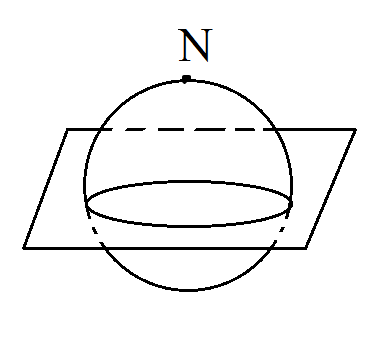
\includegraphics[width = 0.45\linewidth]{5_1.png}}
	\end{figure}


\newpage
%-----------------------------------------------------------------------------
\section{}
	\textbf{Индуцированная топология на подпространстве топологического пространства. Ее описание в метрическом случае. Свойства индуцированной топологии. Замкнутые подмножества и замыкание в индуцированной топологии.}\\
	\\
	$(X, \tau)$ -- топологическое пространство, $Y\subset X$\\
	\textbf{Определение}: $\tau_Y = \{W \cap Y:\ W\in \tau\}$ -- топология, индуцированная на $Y$. В случае метрического пространства $(X,p)$ индуцированная топология продолжается ограничением метрики на $(Y, p_{\mid Y})$\\
	Обозначим: $i_y: Y\rightarrow X, y\rightarrow y$ отображение вложения\\
	\textbf{Теорема}: Характеристическое свойство индуцированной топологии Пусть $Z$ -- топологическое пространство $f: Z\rightarrow Y$, $f$ -- непрерывна $\Leftrightarrow i_y \circ f:\ Z\rightarrow X$ -- непрерывно.
	\begin{figure}[h]
		\center{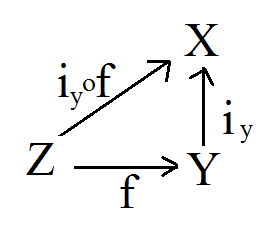
\includegraphics[width = 0.25\linewidth]{6_1.png}}
	\end{figure}\\
	
	\textbf{Теорема}: пусть $\tau$ -- некоторая топология, удовлетворяет свойству из пред. теоремы. Тогда $\tau$ -- слабейшая топология, в которой $i_y$ -- непрерывно. (Если $\tau_1 \subset \tau_2$, то $\tau_1\ \text{Слабее}\ \tau_2$)\\
	\textbf{Доказательство}: 
	\begin{enumerate}
		\item 
		непрерывность $i_Y$. так как $id_Y$ -- непрерывна $\Rightarrow$ по характеристическому свойству и $i_Y$ непрерывна\\
		\begin{figure}[h!]
			\centering
			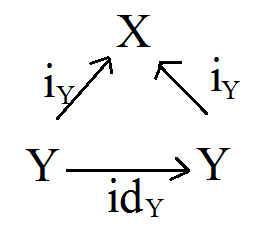
\includegraphics[width = 0.18\linewidth]{6_2.png}
		\end{figure}
		\item 
		Пусть $\tau^{\prime}$ топология на $Y$, в которой $i_Y$ непрерывна $\Rightarrow f$ непрерывна $\Rightarrow \tau \subset \tau^{\prime}$\\
		\begin{figure}[h!]
			\centering
			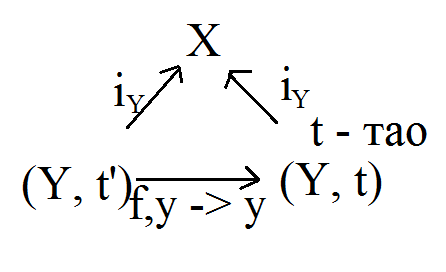
\includegraphics[width = 0.25\linewidth]{6_3.png}
		\end{figure}
	\end{enumerate}
	
	Теорема показывает, что индуцированная топология единственная обладает данным свойством.\\
	\textbf{Следствия}: $X, Y$ -- топологическое пространство, $f:\ X \rightarrow Y$ ограничен $f$ на $A$
	\begin{enumerate}
		\item 
		Если $f$ -- непрерывно, то $\forall A \subset X\ f_{\mid A}:\ A\rightarrow Y$ -- непрерывно
		\item 
		Пусть $B\subset Y,\ B \supset f(x)\ f:\ X\rightarrow Y$ непрерывно $\Leftrightarrow {f\mid}^B:\ X\rightarrow B$ непрерывно
	\end{enumerate}
	\textbf{Доказательство}: 
	\begin{enumerate}
		\item 
		$f_{\mid A} = f\circ i_A$ -- непрерывно
		\item 
		$f = i_B \circ {f\mid}^B$
	\end{enumerate}
	\textbf{Предположения}: 
	\begin{enumerate}
		\item 
		$А$ замкнут в $(Y,\tau_Y) \Leftrightarrow A = B \cap Y$, где $В$ замкнуто в $X$ 
		\item 
		Замыкание $А$ в $(Y,\tau_Y) = \overline{A} \cap Y$
	\end{enumerate}
	\textbf{Доказательство}:
	\begin{enumerate}
		\item 
		След из эквив. $A = B\subset Y \Leftrightarrow Y\setminus A = (X\setminus B)\subset Y\ \forall A\subset Y,\ b\subset X$ 
		\item 
		Замыкание $А$ в $Y = \cup \{C\subset Y:\ c\ \text{замкнуто в Y}\} = \overline{A}\subset Y$, $(A \subset C)$ (Так как $B\cap Y \supset A \Leftrightarrow B\supset A\ \text{для}\ A\subset Y$)
	\end{enumerate}


\newpage
%-----------------------------------------------------------------------------
\section{}
	\textbf{Инициальная топология, порожденная семейством отображений. Свойства инициальной топологии. Произведения топологических пространств. Описание базы произведения в общем случае и в случае конечного числа сомножителей. Универсальное свойство произведения.}\\
	\\
	$X$ -- любое множество; $(X_i, \tau_i)_{i \in I}$ -- семейство, топологическое пространство $(f_i: X\rightarrow X_i)_{i \in I}$ -- семейство отображений.\\
	\textbf{Определение}: инициальная топология на $X$, порожденная семействами $(f_i)$ -- топология с предбазой $\{f_i^{-1}(W_i):\ i \in I,\ W_i \in \tau_i\}$\\
	\\
	\textbf{Теорема} (Характеристическое Свойство)\\ 
	Пусть $Y$ -- топологическое пространство. Отображение $g:\ Y\rightarrow X$ непрерывно относительно $\tau_{in}$\\
	\textbf{Доказательство}:\\
	$g$ -- непрерывно $\Leftrightarrow \forall i \in I,\ \forall W_i \in \tau_i$, $g^{-1}(f^{-1}(W_i))$ открыто $(f_i \circ g)^{-1}(W_i)$ открыто, а значит $f_i \circ g$ непрерывно\\
	\begin{figure}[h]
		\center{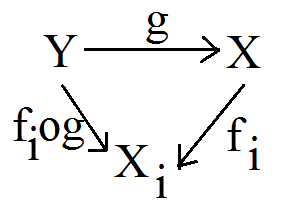
\includegraphics[width = 0.25\linewidth]{7_1.png}}
	\end{figure}	
	\textbf{Определение}: $\prod_{i \in I} = \{X:\ I\rightarrow \bigcup_{i\in I}X_i \mid \forall i\ x(i)\in X_i\}$ -- произведение. Обозначим: $X = \prod_{i\in I},\ x(i) = X_i,\ x = (x_{i})_{i \in I},\ p_i:\ X \rightarrow X_i,\ p_i(x) = x_i$ -- Каноническая проекция $X$ на $X_i$\\
	\textbf{Определение}: Тихоновская топология - инициальная топология на $X$, порожденная $p_i$. Другими словами открытым множеством является произведение открытых подмножеств $x_i$, где конечное число множителей являются собственным подмножеством.\\
	\textbf{Теорема} (универсальное свойство произведения)
	Пусть $Y$ -- топологическое пространство Пусть $\forall i \in I$ задано непрерывно $f_i:\ Y\rightarrow X_i$. Тогда $\exists!$ непрерывное $f:\ Y\rightarrow X$, делающие диаграмму коммутативной $\forall i$.\\
	\textbf{Доказательство}: Определим $f:\ Y\rightarrow X$ формулой $f(y) = f_i(y)$. Оно делает диаграмму коммутативной и является единственным отображением с этим свойством. Непрерывность $f$ из характеристического свойства иницальной топологии.\\
	\begin{figure}[h]
		\centering
		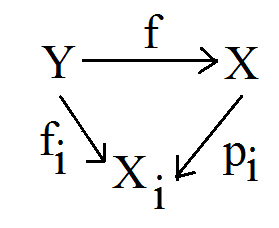
\includegraphics[width = 0.25\linewidth]{7_2.png}
	\end{figure}\\
	\textbf{Теорема} (характеристическое свойство инициальной топологии):\\
	Пусть $\sigma$ -- некоторая топология на $X$, удовлетворяет (1). Тогда $\sigma$ самая слабая топология на $X$, так как $f_i(X, \sigma)-X_i$ непрерывно $\forall i$. Как следствие, $\exists$ только одна такая $\sigma$, а именно $\sigma = \tau_{in}$.\\
	Докажем:\\
	a) $\forall i \in I\ f_i:(X,\sigma) \Rightarrow X_i$ -- непрерывно (см. рис. 1)\\
	б) Если $\sigma^{-1}$ -- некоторая топология на Х, так что $\forall i \in I,\ f_i:(X,\sigma^{-1}) \rightarrow X_i$ -- непрерыно, то $\sigma \subset \sigma^{-1}$. (см.рис.2)
	\begin{figure}[h!]
		\center{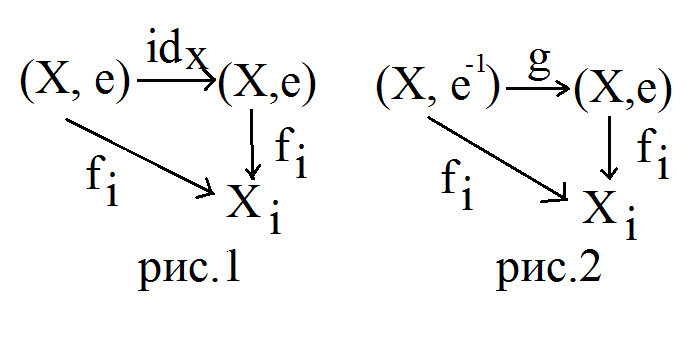
\includegraphics[width = 0.45\linewidth]{7_3.png}}
	\end{figure}\\
	Наблюдения:
	\begin{enumerate}
		\item 
		$\forall i\in I\ \forall U \subset X_i\ p_i^{-1} = \prod_{i\in I} V_j,\ \text{где}\ 
		V_j = 
		\begin{cases}
		X_j\ \text{если}\ x \ne 1\\
		U\ \text{если}\ x = 1\\
		\end{cases}$
		\item 
		для любого конечного $I_0 \subset I,\ \forall $ семейство множеств
		$\{U_i \subset X_i| i\in I_0\}\\
		(*) \cap p_i^{-1}(U_i),\ i \in I_0 = \prod_{j\in I} V_j,\ \text{где} 
		V_j = 
		\begin{cases}
		X_j\ \text{если}\ j\in I_0\\
		U_j\ \text{если}\ j\notin I_0\\
		\end{cases}$
		\item 
		Базу в $X$ образуют множества вида $(*)$ (по всевозможным конечным $I_0\subset I$, всевозможным набором открытых множеств $\{U_i \subset X_i|\ i\in I_0\})$
		\item 
		Если $I = \{1,\ldots ,n\}$, то базу в $X = X_1 \times \ldots \times X_n$ образуют множества вида $U_1 \times \ldots \times U_n$, где $U_i \subset X_i$ открыто для любого $i$
	\end{enumerate} 


\newpage
%-----------------------------------------------------------------------------
\section{}
	\textbf{Метризуемость конечного произведения метризуемых пространств. Декартово произведение семейства непрерывных отображений. Непрерывность поточечных суммы и произведения непрерывных функций со значениями в $\mathbb{R}$. Критерий хаусдорфовости пространства в терминах диагонали. Замкнутость множества точек совпадения двух непрерывных отображений.}\\
	\\
	Пусть $(X_i, p_i)$ -- n метрических пространств, $X = \prod_{i\in I}^n X_i$. Рассмотрим следующую метрику: $p:\ X\times X \rightarrow \left[0;+ \infty\right)\ p(x,y) = \max{p_i(x_i,y_i)}$. Тогда $(Х, р)$ -- метрическое пространство, порождающее топологию произведения.\\
	\textbf{Доказательство}:
	\begin{enumerate}
		\item 
		Заметим, что $\forall x, y \in X:\ p(x,y) < r \Leftrightarrow \forall i\in \{1, 2, \ldots ,n\}\ p_i(x_i,y_i) < r \Rightarrow B_r(x) = \prod_i B_r(x_i) \in \tau$ по седьмому билету (база произведения), следовательно $\tau_p \subset \tau$
		\item 
		Рассмотрим $V = \prod_i B_r(x_i)$ (такие V образуют базу $\tau$).\\
		Выберем произвольно $y\in V$, то есть $y_i\in B_{r_i}(x_i)\ \forall i \Rightarrow \exists \delta_i > 0:\ B_{\delta_i}(y_i) \subset B_{r_i}(x_i)$. Пусть $\delta = \min{\delta_i}$. Тогда $B_\delta (y) = \prod_i B_\delta(y_i) \subset \prod_i B_{\delta_i}(y_i) \subset V$. Поэтому $y$ является внутренней точкой, а значит $V$ открыто в топологии $\tau_p$, следовательно $\tau \subset \tau_p$
		\item
		Откуда $\tau = \tau_p$\\
	\end{enumerate}
	\textbf{Произведение отображений}\\
	\textbf{Определение}: $\prod_i f_i:\ \prod_i X_i \rightarrow \prod_i Y_i,\ f = \prod_i f_i:\ f((x_i)_{i\in I}) = (f_i(x_i))_{i\in I}$ -- произведение семейств $(f_i)$\\
	Предположение: Пусть $(X_i),(Y_i)$ -- семействва топологических пространств, $f_i:\ X_i \rightarrow Y_i$ -- непрерывное отображение. Тогда $\prod_i f_i$ -- тоже непрерывно.\\
	\textbf{Доказательство}: $X = \prod_i X_i,\ Y = \prod_i Y_i,\ f = \prod_i f_i$\\
	\begin{figure}[h!]
		\center{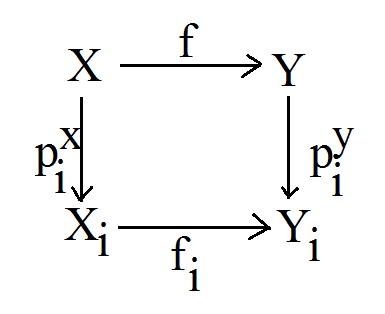
\includegraphics[scale = 0.35]{8_1.png}}
	\end{figure}
	$f \Leftrightarrow p_i^y f$ непрерывно $\forall i \Leftrightarrow f_i p_i^x$ непрерывно $\forall i$, что дано по условию.
	\\
	\\
	$X$ -- топологическое пространство. Обозначение: $X_{+}=X \bigsqcup \{\infty\}$ (дизъюнктивное объединение множеств, а не топологическое  пространств)\\
	\textbf{Обозначение}: ${\tau}_{+}\subset 2^{X_{+}}$ следующим образом: $U\subset \tau_{+} \Leftrightarrow U\subset X$ и открыто в $X$, либо $\infty\subset U$ и $X_{+}\setminus U$ -- замкнуто в $X$ и компактно.\\
	\textbf{Определение}: $(X_{+}, {\tau}_{+})$ -- одноточечная компактификация $X$\\
	\textbf{Определение}: $X, Y$ -- топологические пространства, $f:\ X\Rightarrow Y$\\
	\begin{enumerate}
		\item 
		$f$ -- топологическое вложение $\Leftrightarrow f$ -- гомеоморфизм $X$ на $f(x)$
		\item 
		$f$ -- открытое вложение $\Leftrightarrow f$ -- открыто и является топологическим вложением
	\end{enumerate}
	\textbf{Теорема}: 
	\begin{enumerate}
		\item 
		отображение включения $i_x:\ X\Rightarrow X_{+}$ -- открытое вложение
		\item 
		$X_{+}$ -- компактно
		\item 
		$X_{+}$ хаусдорфово $\Leftrightarrow X$ хаусдорфово и локально компактно
		\item 
		$X$ компактно $\Rightarrow \infty$ -- изолированная точка $X_{+}$ и точка на $X_{+}$ -- топологические дюзъюнктивные объеденения
		\item 
		$X$ плотно в $X_{+} \Leftrightarrow X$ -- не компактно
	\end{enumerate}
	\textbf{Доказательство}: 
	\begin{enumerate}
		\item 
		Из определения ${\tau}_{+}:\ i_x$ -- открыто и инъективно. Докажем непрерывность $i_x$. Пусть $U\subset X_{+}$ открыто. Если $U\subset X$, то и $i_x^{-1}(U) = U$ и $U$ открыто в $X$(по определению ${\tau}_{+})$. Если же $\infty \subset U$, то $i_x^{-1}(U) = U\cap X=X\setminus (X_{+}\setminus U)$ (замкнут в $X$) -- открыто
		\item 
		Пусть $\{U_i \subset I\}$ -- открытое покрытие $X_{+}$. $\exists j\in I$, такое что $\infty \subset U_j$. $X_{+}\subset U_j \cup U_i1 \cup \ldots \cup U_in \Rightarrow X_{+}$ -- компактно
		\item 
		( $\Rightarrow$) $X_{+}$ -- хаусдорфово, тогда $X$ хаусдорфово(см. п.1). Рассмотрим $\forall x \in X \exists$ открытое $U, V \subset X_{+}$, такие что $x\in U, \infty \subset V, U\cap V=\varnothing \Rightarrow U \subset X$ -- открыто, $U\subset X_{+}\setminus V \Rightarrow \overline{U}\subset X_{+}\setminus V$, так как $X_{+}\setminus V$ -- замкнуто. $X_{+}\setminus V$ компактно $\Rightarrow \overline{V}$ -- компактно $\Rightarrow X$ локально компактное\\
		($\Leftarrow$ )Пусть X заусдорфово и локально компактно. Пусть $x,y \in X_{+}$. Ищем открытые $U, V\subset X_{+}$, такие что $X$ хаусдорфово. Если $x, y\in X$, то такие точки $U, V \exists$, так как $X$ хаусдорфово. Пусть $x\in X, y\in \infty$. $\exists$ открытое $U\subset X$, такое что $x\in U$ и $\overline{U}$ -- компактно(где $\overline{U}$ -- замкнуто и в $\infty$). Положим $V = X_{+}\setminus\overline{U} \Rightarrow \infty \in V, X_i\setminus V=\overline{U}$ -- замкнуто в $X$ и компактно $\Rightarrow V$ открыто в $X_{+}$
		\item 
		$X-X_{+}\setminus{\infty}$: $X$ замкнуто в $X$ и компактно $\Rightarrow \{\infty\}$ -- открытое подмножество $X_{+} \Rightarrow \infty$ -- изолированная точка. Из (1) $X$ открытое в $X_{+} \Rightarrow \forall U\subset X_{+} U = (U\cap X)\cup(U\cap\{\infty\}) \Rightarrow U$ открыто в $X_{+} \Leftrightarrow U\cap X$ открыто в $X$. $U\cap \{\infty\}$ открыто в $\{\infty\}$
		\item 
		\begin{enumerate}
			\item
			($\Rightarrow$) Из (4) 
			\item 
			($\Leftarrow$) Пусть $U\subset X_{+}$ открыто, $U \neq \varnothing$. Покажем $U\cap X\neq \varnothing$. В противном случае $U = \{\infty\} \Rightarrow X = X_{+}\setminus U$ компактно, противоречие
		\end{enumerate}		
	\end{enumerate}
	\textbf{Предположение} X, Y-хаусдорфовы топологическое пространства, $f:\ X\Rightarrow Y$ открытое вложение. Рассмотрим $g:\ Y\Rightarrow X_{+},\ g(f(x))=x,\ \forall x\in X,\ g(y) = \infty \forall y\in Y\setminus f(x)$. Тогда $g$ корректно определено и непрерывно.\\
	\textbf{Доказательство}:
	\begin{figure}[h]
		\center{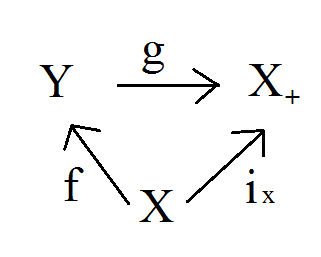
\includegraphics[width = 0.25\linewidth]{18_1.png}}
	\end{figure}
	$f$ -- инъекция $\Rightarrow g$ -- корректно определено. Пусть $U\subset X_{+}$ открыто. Если $U\subset X$, то $g^{-1}(U) \circ f(U)$ -- открыто в $Y$, так как $f$ открыто. Если $\infty\in U$, то положим $K=X_{+}\setminus U,\ K\subset X,\ K$ -- компактно, $g^{-1}(U)$ открыто $\Rightarrow g$ непрерывно\\
	\textbf{Определение}: топологическое пространство $X$ уловлетворяет аксиоме счетности Т1 $\Leftrightarrow \forall x\in X \{x\}$ замкнуто в $X$\\
	Следствие(единственность одноточечной компактификации): $X, Y$ -- топологические пространства, $Y$ -- компактно и хаусдорфово, $f: X\Rightarrow Y$ топологическое вложение , причем $Y\setminus f(x)=\{y_0\}$
	\begin{figure}[h]
		\center{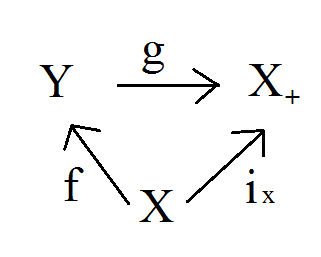
\includegraphics[width = 0.25\linewidth]{18_1.png}}
	\end{figure}
	определим $g:\ Y\Rightarrow X_{+}$ так: $g(f(x)) = x\ \forall x\in X,\ g(y_0) = \infty$. Тогда $g$ -- гомеоморфизм.\\
	\textbf{Доказательство}: $f(x) = Y\setminus \{y_0\},\ \{y_0\}$ замкнуто в $Y \Rightarrow f(x)$ локально компактно и хаусдорфово, $X$ -- гомеоморфно $f(x) \Rightarrow X$ локально компактно и хаусдорфно из окрестности $f(x)$ в $Y \Rightarrow f$ -- открытое вложение. Из предыдущего предложения $\Rightarrow g$ -- непрерывно. По построение $g$ -- биекция. $Y$ -- компактно, $X_{+}$ хаусдорфово (так как $X$ локально компактно и хаусдорфово) $\Rightarrow g$ -- гомеоморфизм.\\
	Примеры:
	\begin{enumerate}
		\item 
		$[0,1) \Rightarrow [0,1] \Rightarrow [0,1) \cong [0,1]$
		\item 
		$(0,1) \Rightarrow S^1,\ t \Rightarrow e^{2\pi i} \Rightarrow {(0,1)}_{+} \cong S^1 \Rightarrow {\mathbb{R}}_{+}\cong S^1$
	\end{enumerate}

\newpage
%-----------------------------------------------------------------------------
\section{}
	\textbf{Финальная топология, порожденная семейством отображений. Cвойства финальной топологии. Дизъюнктные объединения топологических пространств. Универсальное свойство дизъюнктного объединения.}\\
	\\
	$X$ -- множество, $(X_i, {\tau}_i)$ -- семейство топологических пространств, $(f_i: X_i \Rightarrow X)$ -- семейство отображений\\
	Обозначение: ${\tau}_{\text{fin}} = \{U \subset X: \forall i \in I {f_i}^{-1} (U) \subset {\tau}_i \}$\\
	Наблюдение: ${\tau}_{\text{fin}}$ -- топология на $X$\\
	\textbf{Определение}: ${\tau}_{\text{fin}}$ -- финальная топология на $X$, порожденная $(f_i)$\\
	\textbf{Теорема} (характерестическое свойство финальной топологии): $X$ -- множество, снабженное финальной топологией, порожденная семейством $(f_i:\ X_i \Rightarrow X)\ i\in I,\ Y$ -- топологическое пространство\\
	(1) Отображение $g:\ X \Rightarrow Y$ непрерывно $\Leftrightarrow g \circ f_i:\ X_i \Rightarrow Y$ непрерывно $\forall i \in I$\\
	(2) Пусть $\sigma$ -- самая сильна топология на $X$, такая что $\forall i\ f_i:\ X_i \Rightarrow (X, \sigma)$ непрерывно\\
	\textbf{Следствие}: существует только одна такая $\sigma$, а именно $\sigma = {\tau}_{\text{fin}}$\\
	\textbf{Доказательство}: 
	\begin{enumerate}
		\item 
		$(g \circ f)^{-1} = f_i^{-1} (g^{-1}(U))$
		\begin{figure}[h]
			\center{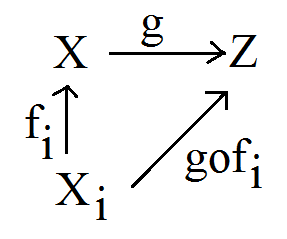
\includegraphics[width = 0.2\linewidth]{9_1.png}}
		\end{figure}
		\item 
		В таком случае $g:\ (X, \tau) \Rightarrow (X, \sigma) |\ x\longmapsto x$ непрерывно, а это значит, что $\sigma \subset \tau$ что и требовалось доказать
		\begin{figure}[h]
			\center{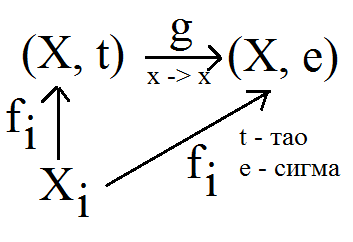
\includegraphics[width = 0.2\linewidth]{9_2.png}}
		\end{figure}\\
	\end{enumerate}
	\textbf{Дизъюнктивное объединение}:\\
	$(X_i) i\in I$-семейство множеств\\
	\textbf{Определение}: $\sqcup X_i = \{(x,i)|\ i\in I,\ x\in X_i\}$-дизъюнктивное объединение семейства $(X_i)$\\
	Обозначение:$\sqcup X_i, e_i:\ X_i \Rightarrow X$\\
	$e_i (x) = (x,i)$ -- каноническое вложение\\
	\textbf{Определение}: топология дизъюнктивного объединения на $X$ -- финальная топология, порожденная семейством канонических вложений\\
	\textbf{Теорема} (универсальное свойство дизъюнктивного объединения):\\
	$(X_i)$ -- семейство топологических пространств $X = \sqcup X_i, Y$ -- топологическое пространство. Тогда для любого семейства непрерывного отобрадения $(f_i:\ X_i \supset Y)$ существует единственное непрерывное $f:\ X\supset Y$, такое что диаграмма коммутативна для любого $i$\\
	\textbf{Доказательство}: определим $f:\ X \Rightarrow Y$ правилом $f(X, i) = f_i (X)\ (x\in X_i,\ i\in I)$. Тогда диаграмма коммутативна для любого $i$, причем $f$ -- единственное отобрадение с этим свойством. непрерывность $f$ из теоремы в начале билета.\\
	\begin{figure}[h]
		\center{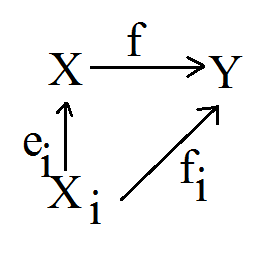
\includegraphics[width = 0.2\linewidth]{9_3.png}}
	\end{figure}

\newpage
%-----------------------------------------------------------------------------
\section{}
	\textbf{Связные топологические пространства. Примеры. Связность отрезка. Основные свойства связных пространств.}\\
	\\
	\textbf{Определение}: топологическое пространство $X$ называется связным, если его нельзя представить в виде $V \cup U$, где $V$ и $U$ -- непустые открытые множества, $V\cap U = \varnothing$. В противном случае несвязным.\\
	Подмножество $Y\subset X$ называется связным, если пространство $Y$ связно в индуцированной топологии.\\
	Утверждение: Пространство $X$ связно тогда, и только тогда, когда $X$ не представимо в виде $A\subset B$, где $А$ и $В$ -- непустые подмножества $X$. Примеры: (Прямая без точки несвязна, антидискретное связно, дискрестное (более чем из 1 очки) несвязно)\\
	Связность отрезка. Отрезок $[a,b]$ на $\mathbb{R}$ связный.\\
	\textbf{Доказательство}:\\
	Предположим противное, тогда $[a,b] = A \subset B$, где $A$ и $B$ -- открытые не пустые подмножества отрезка. В силу открытости $B\ \forall b \in B\ \exists \varepsilon > 0:\ (b -\varepsilon,b] \subset B$ Положим $с = \sup A$. Легко видеть, что $c > a$, (иначе $B = \{a\}$, а значит не открыто), $с < b$\\
	1) Если $c\in A$, то $c$ входит в $А$ с некоторой окрестностью $(c - \sigma,c + \sigma)$. Но тогда есть точка больше с входящая в $А$. Противоречие\\
	2) Если $c\in B$, то $\exists \sigma>0:(c - \sigma,c + \sigma)\subset B$. Тогда лбая точка $a\in A$ дальше от $с$ не менее чем на $\sigma$. противоречие.\\
	\textbf{Cвойства}:\\
	\begin{enumerate}
		\item 
		Непрерывный образ связного пространства связный\\
		\textbf{Доказательство}: Пусть $f(X) = Y = U\subset V$. Тогда $X = f^{-1}(U) \subset f^{-1}(V)$ что и требовалось доказать\\
		\item 
		Пусть $X = U\subset V$. Тогда для любого связного подмножества $A\subset X$ либо $A\subset V$, либо $A\subset U$.\\ \textbf{Доказательство}: $A = (A \cap U)\subset(A\cap V)$, значит в силу связности $А$: либо $A\cap U$, либо $A\cap V$ -- пусто. Пусть $A \cap V = \varnothing$, тогда $V\cap A = A \Leftrightarrow A\subset V$.\\
		\item 
		Если $\{A_i\}_{i\in I}$ -- семейство связных подмножеств $X$, имеющих общую точку, то $\bigcup_i A_i$ -- связно\\
		\textbf{Доказательство}: Будем считать, что $\bigcup_i A_i= X$. Пусть $Х = U\subset V$, выберем общую точку $a:\ a\in A_i \forall i$. Пусть $a\in U \Rightarrow A_i \subset U\ \forall i \Rightarrow \bigcup_i A_i \subset U \Rightarrow V = \varnothing$\\
		\item 
		Если любые две точки $x, y$ из $X$ лежат в связном подмножестве, то $X$ -- связно\\
		\textbf{Доказательство}: Обозначим как $A_{x,y}$ связное подмножество $X$, содержащее $x, y$. Зафиксируем произвольное $x\in X$. Тогда $X = \bigcup_{y\in X} A_{x,y}$. По пункту 3 связно\\
		\item 
		Если $A$ -- связно, $A\subset B \subset \overline{A}$, то $B$ -- связно.\\
		\item 
		Из связности $X_1, X_2, X_3, \ldots, X_n$ следует связность $\prod_i X_i$\\
		\textbf{Доказательство}: докажем для $n = 2$. Пусть $X = X_1,\ Y = X_2$. Пусть $p = (x_1,y_1),\ q = (x_2, y_2)\in X\times Y\\
		A = \{x_1\} \times Y\ \text{гомеоморфно}\ Y \Rightarrow A$ -- связно.\\
		$B = X\times \{y_1\}\ \text{гомеоморфно}\ X \Rightarrow B$ -- связно.\\
		$(x_1,y_2) \in A \cap B \Rightarrow A \cap B \neq \varnothing \Rightarrow A \cup B$ -- связно.\\
		$p,q \in A\cup B \Rightarrow X\times Y$ -- связно.
	\end{enumerate}


\newpage
%-----------------------------------------------------------------------------
\section{}
	\textbf{Линейно связные топологические пространства и их связность. Основные свойства линейно связных пространств. Примеры. Описание связных подмножеств прямой. Теорема «о промежуточном значении».}\\
	\\
	\textbf{Определение}: Пусть $X$ -- топологическое пространство, $x$ и $y$ принадлежат $X$. Пусть из $x$ и $y$ -- непрерывное отображение $f:[0,1] \rightarrow X$, такое что $f(0) = x,\ f(1) = y$\\
	\textbf{Определение}: Множество $X$ называется линейно связным, если для каждой пары точек $x$ и $y$ из $X$ существует пусть из $x$ в $y$.\\
	Предположим: Если $X$ линейно связно, то связно\\
	\textbf{Доказательство}: Зафиксируем $x,y\in X$, пусть $f:[0,1]\rightarrow X$ -- путь из $x$ в $y$. Обозначим $C = f([0,1])$. Так как $x,y \in C$, а $C$ -- связно, то $X$ тоже связно.\\
	Свойства:\\
	\begin{enumerate}
		\item 
		Если $X$ -- линейно связно, $f:\ x\rightarrow Y$ -- непрерывно, то $f(X)$ линейно связно.\\
		\item
		Если $\{A_i\}_{i\in I}$ -- семейство линейно связных подмножеств $X$, имеющих общую точку, то $\prod_i A_i$ -- линейно связно
		\item 
		Если любые две точки $x$ и $y$ из $X$ лежат в линейно связном подмножестве, то $X$ линейно связно
		\item 
		Произведение линейно связных пространств линейно связно
	\end{enumerate}
	\textbf{Доказательства}:
	\begin{enumerate}
		\item 
		Произвольно выберем $x,y \in f(X)$. В силу линейной связности $X$ между точками $x^{-1} \in f^{-1}(y)$ существует путь $g:[0,1] \rightarrow X$. Значит, между $x$ и $y$ существует путь $f\circ g:\ [0,1] \rightarrow f(X)$\\
		\item 
		Пусть $a$ -- общая точка множеств $A_i$. $\forall x,\ y \in \bigcup_i A_i.\ x\in A_{i_x},\ y\in A_{i_y},\ a\in A_{i_x}, A_{i_y} \exists f_x \text{из х в а},\ f_y \text{из а в у}$ Очевидно что есть функция которая при $х > а$ ведет себя как $f_x$, а при меньших как $f_y$\\ 
		\item 
		Если любые две точки лежат в линейно связном подмножестве, то между ними существует путь, а значит и само множество линейно связано.\\
		\item 
		Рассмотрим семейство линейно связных пространств $\{X_i\}_{i\in I}$. Выберем произвольные точки $p = (p_i)_{i\in I},\ q = (q_i)_{i\in I} \in \prod_{i\in I} X_i$. Пусть $f_i$ путь из $p_i$ в $q_i$. Тогда путем из $p$ в $q$ будет $\prod_{i\in I} X_i$
	\end{enumerate}
	\textbf{Примеры}: $X$ -- нормированное простраство. 
	\begin{enumerate}
		\item 
		Любое выпуклое подмножество $U\subset X$-- линейно связно
		\item 
		Если $\dim_R X>1$, то $X\setminus\{0\}$ -- связно
		\item 
		$n$-мерный тор $T^n = S^1\times \ldots \times S^1 \text{(n раз)}$ -- линейно связный
	\end{enumerate}
	Связные подмножества прямой:\\
	Помножество $a\subset \mathbb{R}$ называется промежутком, если (сами знаете. интервал отрезок, два полотрезка и пустое множество)\\
	Следующие свойства эквивалентны 
	\begin{enumerate}
		\item $А$ связно 
		\item $А$ линейно связно 
		\item $А$ промежуток		
	\end{enumerate}
	$2 \rightarrow 1$ доказывали выше, $3 \rightarrow 2$ очевидно. Докажем $1 \rightarrow 3$\\
	1) Предположим, что А ограничено. $а = \text{inf} A,\ b=\sup A$, тогда $a \subset[a,b]$. Покажем, что $(a,b)\subset A$. Пусть $(a,b) \in A$. Тогда существует точка $c\in (a,b),\ c\in A$\\
	Обозначим $U = A\cap ( -\infty, c),\ V = A\cap (c,+ \infty)$. $U, V$ -- открытые непустые множества, что протеворечит связности. $\Rightarrow (a,b)\subset A \subset [a,b]$.
	2) Если не ограничено, то либо совпадает с $\mathbb{R}$, либо нет какой-то $с$, далее действуем аналогично.
	

\newpage
%-----------------------------------------------------------------------------
\section{}
	\textbf{Связные и линейно связные компоненты, их свойства, примеры. Локально линейно связные пространства и свойства их компонент.}\\
	\\
	\textbf{Определение}: Связная компонента пространства $X$-максимальное по включению связное подмножество $X$\\
	\textbf{Теорема}: 
	\begin{enumerate}
		\item 
		Связные компоненты образуют разбиение $X$ (то есть их объединение-все пространство $X$ и любая связная компонента $X_1,X_2$ либо $X_1 = X_2$, либо $X_1 \cap X_2 = \varnothing$)
		\item 
		$\forall x\in X$ связная компонента $X$, содержащая $x$ равна $C(x)=\cup \{A\subset X |\ A\ \text{связно},\ x\in A\}$
		\item 
		Каждое непустое связное подмножество $X$ содержится ровно в одной связной компоненте 
		\item 
		Связные компоненты замкнуты в $X$
	\end{enumerate}
	\textbf{Доказательство}:\\
	(1),(2) Пусть $X_1, X_2 \subset X$-связные компоненты, $X_1 \cap X_2 \neq \varnothing \Rightarrow X_1 \cup X_2$ связно $\Rightarrow X_1=X_1 \cup X_2=X_2$\\
	Зафиксируем $x\in X$ и определим $C(x)$ равенством (2). $C(x)$ связно, и является наибольшим связным подмножеством $X$, содержащим $x \Rightarrow C(x)$-связная компонента\\
	(3) Пусть $A\subset X,\ A \neq \varnothing$. $A$ связно. В силу (1) существует связная компонента $B\subset X$, такая что $A\cap B \neq \varnothing \Rightarrow A\cup B$ связно $\Rightarrow B=A\cup B \Rightarrow A\subset B$\\
	(4) $A$-связная компонента $\Rightarrow \overline{A}$ связно $\Rightarrow A = \overline{A}$ что и требовалось доказать\\
	\\
	\textbf{Следствие}: Если X состоит из конечного числа связных компонент, то они открыты в $X$\\
	\textbf{Доказательство}: $X=X_1 \cup X_2 \cup \ldots \cup X_n$ -- разбиение на связные компоненты $X\slash X_1=X_2 \cup \ldots X_n \Rightarrow X_1$ открыто что и требовалось доказать\\
	\textbf{Пример}: Связные компоненты $\mathbb{R} \slash \{0\}$-это $( - \infty , 0)$ и $(0, + \infty)$\\
	$X_1,X_2$ -- непустые связные пространства $\Rightarrow X_1$ и $X_2$ -- связные компоненты $X_1 \sqcup X_2$\\
	$X$ -- дискретное пространство, $\mathbb{Q}$ или канторово множество. Связные компоненты $X$-одноточечные подмножества\\
	\\
	\textbf{Определение}: Линейно связная компонента $X$-максимальное линейное связное подмножество $X$\\
	\textbf{Теорема}:
	\begin{enumerate}
		\item 
		Линейно связные компоненты образуют разбиение $X$
		\item 
		Для любой точки $x\in X$ линейно связная компонента, содержащая ее, равна\\ $PC(x)=\cup \{A\subset X| A\ \text{-- линейно связно}\  x\in A\}$
		\item 
		Каждое непустое линейно связное подмножество $X$ содержится ровно в одной линейно связной компоненте
	\end{enumerate}
	\textbf{Доказательство}: аналог доказательства прошлой теоремы, однако линейно связные компоненты $X$ не всегда замкнуты в $X$.\\
	\textbf{Пример} $X=\{(x,\sin{\frac{1}{x}}):\ 0 \textless \leqslant 1\} \cup \{(0,y):- 1\leqslant y \leqslant 1\} \subset \mathbb{R}^2$\\
	\textbf{Определение}: Пространство $X$ локально линейно связно, если $\forall x\in X$ в любой окрестности $x$ содержится линейно связная окрестность $x$. Эквивалентно, у $X$ есть база, состоящая из линейно связных множеств\\
	\textbf{Пример} открытые подмножества нормированного пространства локально линейно связны\\
	\textbf{Предположение} Пусть $X$-локально линейно связное пространство. Тогда каждая линейно связная компонента $X$ открыта в $X$ и является связной компонентой. В частности,$X$ связно $\Leftrightarrow X$ линейно связно\\
	\textbf{Доказательство}: Пусть $A\subset X$-линейно связная компонента, $\forall x\in A$ существует линейно связная окрестность $U_x(x\in U_x) \forall A\cup U_x$ линейно связно $\Rightarrow A=A\cup U_x$, то есть $U_x \subset A \Rightarrow A$ открыто\\
	Пусть $B\subset X$-связная компонента, $A\subset B\\
	B\slash A$-объединение линейно связных компонент $X$, содержащихся в $B$ и отличных от $A$. A открыто, $B\slash A$ открыто как объединение открытых множеств, $A \neq \varnothing \Rightarrow B\slash A=\varnothing$ в силу связности$ B. A=B$ что и требовалось доказать
	

\newpage
%-----------------------------------------------------------------------------
\section{}
	\textbf{Компактные топологические пространства. Критерий компактности в терминах замкнутых множеств. Критерий компактности подпространства (в терминах покрытий множествами, открытыми в топологии объемлющего пространства).}\\
	\\
	\textbf{Определение}: Пусть $X$ -- множество. $U \subset 2^{X},\ U$ -- покрытие $Y\subset X \Leftrightarrow Y \subset U$\\
	\textbf{Определение}: Подпокрытие покрытия $U$ -- покрытие $V$ множества $Y$, такое что $V\subset U$\\
	Если $X$ -- топологическое пространство, то покрытие $U$ называется открытым, когда состоит из открытых множеств\\
	\textbf{Определение}: Топологическое пространство $X$ называется компактным, если каждое его открытое покрытие содержит конечное открытое подпокрытие.\\
	\textbf{Предположение} $X$ -- топологическое пространство. Подпространство $Y \subset X$ -- компактно(в индуцированной топологии) $\Leftrightarrow$ любое покрытие множества $Y$, состоящее из множеств открытых в $X$, имеет конечное подпокрытие\\
	\textbf{Доказательство}: $Y$ -- компактно $\Rightarrow$ для любого покрытия $U$ существует конечное подпокрытие $V$. Пусть $W$ -- покрытие $Y$ открытыми в $X$, такое что $\forall F_{Y} \in U\ \exists F_{X} \in W$, такое что $F_{Y} = F_{X}\cap Y$. Тогда заметим, что для конечного покрытия $V$ существует конечный набор открытых в $W$, который так же является покрытием $Y$\\
	\textbf{Задача}: Доказать компактность замкнутого куба $[a,b]^n \subset \mathbb{R}$\\
	\textbf{Доказательство}: Докажем сначала для $n = 1$. Это просто отрезок на прямой. Пусть существует покрытие отрезка, из которого нельзя выделить конечное подпокрытие. Разделим отрезок пополам. Выберем ту часть, которую нельзя конечно покрыть. Разделим ее пополам, выберем из этих двух половин ту часть, которую нельзя покрыть и тд. Получим последовательность вложенных отрезков, а они сходятся к точке. Она принадлежит какому-то интервалу. Пусть расстояние от точки до ближайшего конца интервала $r$. Тогда существует такой отрезок, длины меньше $r$, из этой последовательности вложенных отрезков, который очень даже покрывается этим интервалом, а по предположению не покрывался конечно.\\
	\begin{enumerate}
		\item 
		$n = 2$ аналогично $n = 1$, но берем один из четырех квадратов и смотрим на круги
		\item 
		$n = 3$ -- рассматриваем вложенные 3-мерные кубы и 3-мерные шары
		\item 
		$n$ -- рассматриваем $n$-мерные вложенные кубы и $n$-мерные шары
	\end{enumerate}


\newpage
%-----------------------------------------------------------------------------
\section{}
	\textbf{Основные свойства компактных топологических пространств (связь компактности подпространств и их замкнутости, свойства непрерывных отображений из компактного пространства). Основное свойство функций на компактном пространстве со значениями в $\mathbb{R}$.}\\
	\\
	Свойства компактных пространств:\\
	\begin{enumerate}
		\item 
		$X,Y$ -- топологические пространства, $X$ -- компакт, $f: X\Rightarrow Y$ непрерывно. Тогда $f(X)$ -- компакт
		\item 
		$X$ -- компактное пространство, $Y \subset X$ замкнуто $\Rightarrow Y$ -- компакт
		\item 
		$X$ -- хаусдорфово, $Y \subset X$ -- компакт $\Rightarrow Y$ -- замкнуто
		\item 
		$X$ -- компактное пространство, $Y$ -- хаусдорфово, $f:\ X\Rightarrow Y$ непрерывно. Тогда $f$ замкнуто
		\item 
		Если $X$ -- компактное топологическое пространство, $Y$ -- хаусдорфово пространство, $f:\ X\Rightarrow Y$ биекция. Тогда $f$ -- гомеоморфизм
	\end{enumerate}
	\textbf{Доказательство}: 
	\begin{enumerate}
		\item 
		Считаем, что $Y = f(X)$. Пусть $U$ -- открытое покрытие $Y$. Тогда $V$, прообраз $U$ -- открытое покрытие $X$. Так как $X$ -- компакт, то из $V$ можно выделить конечное подпокрытие, а его образ это конечное подпокрытие покрытия $U$, значит $Y$ -- компакт
		\item 
		Пусть $U$ -- покрытие $Y$ множествами, открытыми в $X$. $U\cup \{X\slash Y\}$ -- открытое покрытие $X$. $X$ -- компакт, следовательно $\exists V_1,\ldots, V_n \in U$, такое что $X = V_1 \cup \ldots \cup V_n \cup \{X\slash Y\}$, значит $Y \subset V_1 \cup \ldots \cup V_n$
		\item 
		Пусть $Y$ компактно. Пусть $x\in X\slash Y$\\
		Из хаусдорфовости $\forall y\in Y \exists$ окрестности $y\in U_y$ и $x\in U_x, U_y\cap U_x = \varnothing\ \{U_y: y\in Y\}$ -- покрытие $Y$, открытыми в $X$. Следователно $\exists y_1,\ldots,y_n \in Y:\ Y\subset U_1 \cup \ldots \cup U_n$. Обозначим $V = V_{y_1} \cap \ldots \cap V_{y_n}$ -- окрестности точки $x$ и $V\cap Y = \varnothing$, следовательно $x$ не лежит в $\overline{Y}$, то есть $y = \overline{Y}$
		\item 
		B $\subset X$ -- замкнутое подпространство. В силу (2) оно компактно, в силу (1) $f(B)$ -- компактно, в силу (3) $f(B)$ -- замкнуто
		\item 
		Частный случай (4)
	\end{enumerate}
	\textbf{Определение}: $X$ ограничено, если $\text{diam} X \textless \infty$, где $\text{diam} X=\sup \{\rho(x,y): x,y \in X\} \in [0,+ \infty)$\\
	\textbf{Предположение} $X$ -- компакт, $X \neq \varnothing.\ f\in C(X, \mathbb{R}) \Rightarrow f$ ограничено и достигает наибольшего и наименьшего значений\\
	\textbf{Доказательство}: $f(X) \subseteq \mathbb{R},\ f(X)$ компактен ((1) свойство). $A \subseteq \mathbb{R}$ -- компактное $\Leftrightarrow A$ замкнуто и ограничено (см. Теорему). Значит, $f(X)$ замкнуто и ограничено. В частности, $f$ достигает на $x \sup$ и $\inf$
	

\newpage
%-----------------------------------------------------------------------------
\section{}
	\textbf{Центрированные семейства множеств и их свойства. Теорема Тихонова о компактности произведения. Критерий компактности подмножества в $\mathbb{R}^n$.}\\
	\\
	\textbf{Определение}: Пусть $X$ -- произвольное множество, $F\subset 2^{X},\ F$ -- центрированное $\Leftrightarrow$ для любых конечных $F_0 \subset F:\ \cap F_0 \neq \varnothing$ (Семейство, в котором пересечения конечных подсемейств не пусты)\\
	\textbf{Предположение} топологическое пространство $X$ -- компактно $\Leftrightarrow$ каждое центрированное семейство замкнутых подмножеств имеет непустое пересечение.\\
	\textbf{Доказательство}: заметим, что для любого $F\subset 2^{X}$ верно следующее:
	\begin{enumerate}
		\item
		$\cap F=\varnothing \Leftrightarrow \{X\slash K: K \in F\}$ -- покрытие $X$
		\item
		$F$ -- центрированное $\Leftrightarrow$ для любого конечного $F_0 \subset F:\{X\slash K: K\in F_o\}$ не покрывает $X$
		\item 
		$(\Rightarrow)$ Пусть какое-то центрированное семейство $F$ имеет пустое пересечение. Дополнение $X$ до него это покрытие. Но мы не можем выделить конечное подпокрытие, так как любое конечное подпокрытие -- это дополнение до конечного подмножества $F_0 \subset F$, а его пересечение по определению непусто
		\item 
		$(\Leftarrow)$ Пусть $X$ не компакт. Тогда существует покрытие $U$, такое что любое конечное $V\subset U$ -- не покрытие. Рассмотрим дополнение $F$ к $U$ и $F_0$ к $V$. Заметим, что $V\subset U \Rightarrow F_o \subset F и F_0$ -- конечное, $\cap F_0 \neq \varnothing (V$ не покрытие). То есть $F$ -- центрированное семейство, имеющее пустое пересечение(дополнение к нему -- покрытие). 
	\end{enumerate}
	\textbf{Теорема}: $X \subset \mathbb{R}^n$ компактно $\Leftrightarrow X$ замкнуто и ограничено в евклидовой метрике\\
	\textbf{Доказательство}:\\
	($\Rightarrow$) $X$ -- компактно, следовательно $X \subset \cup B_r (0) \Rightarrow \exists r_1,\ldots, r_k:\ X\subset B_{r_1} (0) \cup\ldots \cup B_{r_k}(0) = B_r(0),\ \text{где}\ r = \max(r_1,\ldots ,r_k).\ X\subset B_r(0)$, следовательно $X$ -- ограничено. $X$ -- замкнуто из 3 свойства\\
	($\Leftarrow$) существует замкнутый куб $C\subset \mathbb{R}^n$, такой что $X\subset C.\ C$ -- компакт((1) свойство). $X$ замкнуто в $C$, следовательно $X$ -- компакт ((2) свойство)\\
	

\newpage
%-----------------------------------------------------------------------------
\section{}
	\textbf{Локально компактные топологические пространства. Примеры и контрпримеры. Локальная компактность конечных произведений, замкнутых и открытых подмножеств.}\\
	\\
		\textbf{Определение}: топологическое пространство X локально компактно $\Leftrightarrow \forall x \in X\ \exists$
	окрестность $U \ni x$, такая что $U$ компактна\\
	\textbf{Пример} 
	\begin{enumerate}
		\item 
		компактно $\Rightarrow$ локально компактно
		\item 
		дискретное $\Rightarrow$ локально компактно
		\item 
		$\mathbb{R}^n$ локально компактно
		\item 
		$\mathbb{Q}$ не локально компактно
	\end{enumerate}
	Действительно $\forall $ интервала $(a,b)$ замыкание $(a,b)\cap \mathbb{Q}$ в $\mathbb{Q}$ равно $[a,b]\cap \mathbb{Q}$-локально (так как замкнуто в $\mathbb{R}$)\\
	\\
	\textbf{Предложение 1}: $X_1, \ldots , X_n$ локально компактно $\Rightarrow \overset{n}{\underset{i = 1}{\prod}} x_i$ локально компактно\\
	\textbf{Доказательство}: Пусть $X = (X_1,\ldots , X_n)\in \overset{n}{\underset{i = 1}{\prod}} X_i\ \forall i = 1,\ldots,n\ \exists$ окрестность $U_i(x_i\in U_i) U_i \subset X_i$, такая что $\overline{U_i}$ -- компактно\\
	\\
	\textbf{Предложение 2}: $X$ -- локально компактно, $Y \subset X$-замкнуто $\Rightarrow Y$ -- локально компактно\\
	\textbf{Доказательство}: Пусть $y\in Y\ \exists$ открытое $U\subset X$, такая что $y\in U$, $\overline{U}$ -- компактно. Тогда $U\cap Y$ окрестность $y$ в $Y$, замыкание $U\cap Y$ в $Y$ равно $\overline{U}\cap Y$, $\overline{U}\cap Y$ замкнуто в $X \Rightarrow$ оно замкнуто в $\overline{U} \Rightarrow$ оно компактно\\
	\\
	\textbf{Предложение 3}: $X$ -- хаусдорфово локально компактное пространство, $Y\subset X$ открыто $\Rightarrow Y$ локально компактно\\
	\\
	\textbf{Лемма 1}: $X$ -- хаусдорфово топологическое пространство, $Y\subset X$ компактно, $x\in X\setminus Y$, тогда $\exists$ открытые $U, V\subset X$, такие что $Y\subset V, X\subset U, U\cup V=\varnothing$ \\
	\textbf{Доказательство}: аналогично доказательству замкнутости $Y$\\
	\textbf{Лемма 2}: $X$ -- хаусдорфово локально компактное пространство. Тогда $\forall x\in X$, $\forall $ окрестности $U(X\subset U) \exists$ окрестность $V(x\in V)$, такое что $\overline{V}\subset U$ и $\overline{V}$ -- компактно\\
	\textbf{Доказательство}: Пусть $W$ -- окрестность $x$, такая что $\overline{W}$ -- компактно. Обозначим $K=\overline{W}\setminus U$, $K$-замкнутое подмножество $\overline{W} \Rightarrow K$ -- компактно, $x$ не принадлежит $K$. По Лемме 1, $\exists$ окрестности $U^{\prime},\ V^{\prime} \subset X$, такие что $K\subset U^{\prime},\ x\in V^{\prime},\ U^{\prime}\cap V^{\prime} = \varnothing$.\\
	Обозначим $V = W\cap V^{\prime},\ V$ -- окрестность $X$, $\overline{V}\subset\overline{W} \Rightarrow \overline{V}$ -- компактно\\
	$\overline{V}\subset(\overline{W}\cap\overline{V^{\prime}})\subset(\overline{W}\cap(\overline{X\setminus U^{\prime}}) = \overline{W}\cap (X\setminus U^{\prime}) = (U \text{-- открытое})\qquad \overline{W}\setminus V^{\prime} \subset \overline{W}\setminus K \subset U$ \\
	\textbf{Доказательство}: Пусть $y\in Y$. В силу Леммы 3 $\exists$ окрестность $V(y\in V)$, такая что $\overline{V}\cap Y,\ V\cap Y = V \Rightarrow V$ -- открытое подмножество $Y,\ \overline{V} = \overline{V}\cap Y$ -- компактно

\newpage
%-----------------------------------------------------------------------------
\section{}
	\textbf{Одноточечная компактификация, ее основные свойства (компактность, критерий хаусдорфовости$\ldots$). «Единственность» одноточечной компактификации. Примеры одноточечных компактификаций.}\\
	\\
	$X$ -- топологическое пространство. Обозначение: $X_{+}=X \bigsqcup \{\infty\}$ (дизъюнктивное объединение множеств, а не топологическое  пространств)\\
	\textbf{Обозначение}: ${\tau}_{+}\subset 2^{X_{+}}$ следующим образом: $U\subset \tau_{+} \Leftrightarrow U\subset X$ и открыто в $X$, либо $\infty\subset U$ и $X_{+}\setminus U$ -- замкнуто в $X$ и компактно.\\
	\textbf{Определение}: $(X_{+}, {\tau}_{+})$ -- одноточечная компактификация $X$\\
	\textbf{Определение}: $X, Y$ -- топологические пространства, $f:\ X\Rightarrow Y$\\
	\begin{enumerate}
		\item 
		$f$ -- топологическое вложение $\Leftrightarrow f$ -- гомеоморфизм $X$ на $f(x)$
		\item 
		$f$ -- открытое вложение $\Leftrightarrow f$ -- открыто и является топологическим вложением
	\end{enumerate}
	\textbf{Теорема}: 
	\begin{enumerate}
		\item 
		отображение включения $i_x:\ X\Rightarrow X_{+}$ -- открытое вложение
		\item 
		$X_{+}$ -- компактно
		\item 
		$X_{+}$ хаусдорфово $\Leftrightarrow X$ хаусдорфово и локально компактно
		\item 
		$X$ компактно $\Rightarrow \infty$ -- изолированная точка $X_{+}$ и точка на $X_{+}$ -- топологические дюзъюнктивные объеденения
		\item 
		$X$ плотно в $X_{+} \Leftrightarrow X$ -- не компактно
	\end{enumerate}
	\textbf{Доказательство}: 
	\begin{enumerate}
		\item 
		Из определения ${\tau}_{+}:\ i_x$ -- открыто и инъективно. Докажем непрерывность $i_x$. Пусть $U\subset X_{+}$ открыто. Если $U\subset X$, то и $i_x^{-1}(U) = U$ и $U$ открыто в $X$(по определению ${\tau}_{+})$. Если же $\infty \subset U$, то $i_x^{-1}(U) = U\cap X=X\setminus (X_{+}\setminus U)$ (замкнут в $X$) -- открыто
		\item 
		Пусть $\{U_i \subset I\}$ -- открытое покрытие $X_{+}$. $\exists j\in I$, такое что $\infty \subset U_j$. $X_{+}\subset U_j \cup U_i1 \cup \ldots \cup U_in \Rightarrow X_{+}$ -- компактно
		\item 
		( $\Rightarrow$) $X_{+}$ -- хаусдорфово, тогда $X$ хаусдорфово(см. п.1). Рассмотрим $\forall x \in X \exists$ открытое $U, V \subset X_{+}$, такие что $x\in U, \infty \subset V, U\cap V=\varnothing \Rightarrow U \subset X$ -- открыто, $U\subset X_{+}\setminus V \Rightarrow \overline{U}\subset X_{+}\setminus V$, так как $X_{+}\setminus V$ -- замкнуто. $X_{+}\setminus V$ компактно $\Rightarrow \overline{V}$ -- компактно $\Rightarrow X$ локально компактное\\
		($\Leftarrow$ )Пусть X заусдорфово и локально компактно. Пусть $x,y \in X_{+}$. Ищем открытые $U, V\subset X_{+}$, такие что $X$ хаусдорфово. Если $x, y\in X$, то такие точки $U, V \exists$, так как $X$ хаусдорфово. Пусть $x\in X, y\in \infty$. $\exists$ открытое $U\subset X$, такое что $x\in U$ и $\overline{U}$ -- компактно(где $\overline{U}$ -- замкнуто и в $\infty$). Положим $V = X_{+}\setminus\overline{U} \Rightarrow \infty \in V, X_i\setminus V=\overline{U}$ -- замкнуто в $X$ и компактно $\Rightarrow V$ открыто в $X_{+}$
		\item 
		$X-X_{+}\setminus{\infty}$: $X$ замкнуто в $X$ и компактно $\Rightarrow \{\infty\}$ -- открытое подмножество $X_{+} \Rightarrow \infty$ -- изолированная точка. Из (1) $X$ открытое в $X_{+} \Rightarrow \forall U\subset X_{+} U = (U\cap X)\cup(U\cap\{\infty\}) \Rightarrow U$ открыто в $X_{+} \Leftrightarrow U\cap X$ открыто в $X$. $U\cap \{\infty\}$ открыто в $\{\infty\}$
		\item 
		\begin{enumerate}
			\item
			($\Rightarrow$) Из (4) 
			\item 
			($\Leftarrow$) Пусть $U\subset X_{+}$ открыто, $U \neq \varnothing$. Покажем $U\cap X\neq \varnothing$. В противном случае $U = \{\infty\} \Rightarrow X = X_{+}\setminus U$ компактно, противоречие
		\end{enumerate}		
	\end{enumerate}
	\textbf{Предположение} X, Y-хаусдорфовы топологическое пространства, $f:\ X\Rightarrow Y$ открытое вложение. Рассмотрим $g:\ Y\Rightarrow X_{+},\ g(f(x))=x,\ \forall x\in X,\ g(y) = \infty \forall y\in Y\setminus f(x)$. Тогда $g$ корректно определено и непрерывно.\\
	\textbf{Доказательство}:
	\begin{figure}[h]
		\center{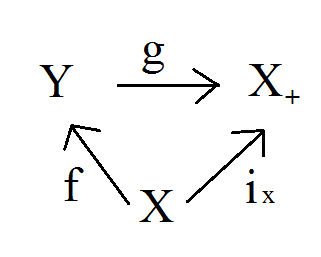
\includegraphics[width = 0.25\linewidth]{18_1.png}}
	\end{figure}
	$f$ -- инъекция $\Rightarrow g$ -- корректно определено. Пусть $U\subset X_{+}$ открыто. Если $U\subset X$, то $g^{-1}(U) \circ f(U)$ -- открыто в $Y$, так как $f$ открыто. Если $\infty\in U$, то положим $K=X_{+}\setminus U,\ K\subset X,\ K$ -- компактно, $g^{-1}(U)$ открыто $\Rightarrow g$ непрерывно\\
	\textbf{Определение}: топологическое пространство $X$ уловлетворяет аксиоме счетности Т1 $\Leftrightarrow \forall x\in X \{x\}$ замкнуто в $X$\\
	Следствие(единственность одноточечной компактификации): $X, Y$ -- топологические пространства, $Y$ -- компактно и хаусдорфово, $f: X\Rightarrow Y$ топологическое вложение , причем $Y\setminus f(x)=\{y_0\}$
	\begin{figure}[h]
		\center{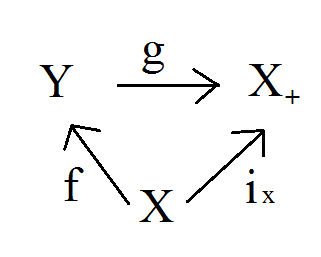
\includegraphics[width = 0.25\linewidth]{18_1.png}}
	\end{figure}
	определим $g:\ Y\Rightarrow X_{+}$ так: $g(f(x)) = x\ \forall x\in X,\ g(y_0) = \infty$. Тогда $g$ -- гомеоморфизм.\\
	\textbf{Доказательство}: $f(x) = Y\setminus \{y_0\},\ \{y_0\}$ замкнуто в $Y \Rightarrow f(x)$ локально компактно и хаусдорфово, $X$ -- гомеоморфно $f(x) \Rightarrow X$ локально компактно и хаусдорфно из окрестности $f(x)$ в $Y \Rightarrow f$ -- открытое вложение. Из предыдущего предложения $\Rightarrow g$ -- непрерывно. По построение $g$ -- биекция. $Y$ -- компактно, $X_{+}$ хаусдорфово (так как $X$ локально компактно и хаусдорфово) $\Rightarrow g$ -- гомеоморфизм.\\
	Примеры:
	\begin{enumerate}
		\item 
		$[0,1) \Rightarrow [0,1] \Rightarrow [0,1) \cong [0,1]$
		\item 
		$(0,1) \Rightarrow S^1,\ t \Rightarrow e^{2\pi i} \Rightarrow {(0,1)}_{+} \cong S^1 \Rightarrow {\mathbb{R}}_{+}\cong S^1$
	\end{enumerate}

\newpage
%-----------------------------------------------------------------------------
\section{}
	\textbf{Понятия мажорирования и эквивалентности норм на векторном пространстве. Критерий мажорирования одной нормы другой. Теорема об эквивалентности норм на конечномерном векторном пространстве.}\\
	\\
	Пусть $X$ -- векторное пространство над $\mathbb{K}$, где $\mathbb{K}$ -- это $\mathbb{R}$ или $\mathbb{C}$\\
	\textbf{Определение}: Функция $X \Rightarrow [0,+ \infty),\ x \Rightarrow ||x||$ называется нормой на $X$:
	\begin{enumerate}
		\item 
		$||\lambda x|| = |\lambda| ||x||$, где $\lambda \in \mathbb{K},\ x\in X$
		\item 
		$||x|| + ||y|| \geqslant ||x + y||\ (x,y \in X)$
		\item 
		$||x|| \textgreater 0,\ \forall x \neq 0$
	\end{enumerate}
	Пусть $||\cdot||^{\prime}$ и $||\cdot||^{\prime \prime}$ -- нормы на $X$, порождающие топологии $\tau^{\prime}$ и $\tau^{\prime \prime}$ соответственно\\
	\textbf{Определение}: Норма $||\cdot||^{\prime}$ мажорируется нормой $||\cdot||^{\prime \prime}$ (обозн: $||\cdot||^{\prime} \prec ||\cdot||^{\prime \prime}) \Leftrightarrow \tau^{\prime} \subset \tau^{\prime \prime}$\\
	$||\cdot||^{\prime}$ эквивалентна $||\cdot||^{\prime \prime} \Leftrightarrow \tau^{\prime}=\tau^{\prime \prime}$\\
	\textbf{Предположение}: Следующие свойства эквивалентны:
	\begin{enumerate}
		\item 
		$||\cdot||^{\prime} \prec ||\cdot||^{\prime \prime}$
		\item 
		$\exists C \textgreater 0$, такое что $\forall x\in X\ ||x||^{\prime} \leqslant C||x||^{\prime \prime}$
	\end{enumerate}
	\textbf{Доказательство}: $||\cdot||^{\prime} \prec ||\cdot||^{\prime \prime} \Leftrightarrow$ отображение $(X, \tau^{\prime \prime})\Rightarrow (X, \tau^{\prime})$, $x\Rightarrow x$ непрерывно\\
	$\Leftrightarrow из x_n \to x в \tau^{\prime \prime}$ следует, что $x_n \to x в \tau^{\prime}$\\
	\\
	$(2) \Rightarrow (1)$ $x_n \to x d \tau^{\prime \prime}$ то есть $||x_n - x||^{\prime \prime} \to 0\quad \exists ||x_n - x||^{\prime} \leqslant C||x_n - x||^{\prime \prime} \to 0$\\
	$(1) \Rightarrow (2)$ Пусть 2 не выполнено $\forall n \in \mathbb{N}\quad \exists x_n \in X$, такое что $||x_n||^{\prime} \textgreater n^2 ||x_n||^{\prime \prime}$\\
	\\
	\textbf{Обозначим}: $y_n = \frac{x_n}{n||x_n||^{\prime \prime}} \Rightarrow ||y_n||^{\prime \prime}=\frac{1}{n} \to 0\\
	y_n \to 0$ в $\tau^{\prime \prime}\\
	||y_n||^{\prime}=\frac{||x_n||^{\prime}}{n||x_n||^{\prime \prime}} \textgreater n \Rightarrow y_n \nrightarrow 0$ в $\tau^{\prime}$ (и вообще не сходится, так как неограничен), противоречие\\
	\textbf{Следствие}: $||\cdot||^{\prime} \sim ||\cdot||^{\prime \prime}\ \exists c,\ C \textgreater 0$, такое что $\forall x\in X\ c||x||^{\prime \prime} \leqslant ||x||^{\prime} \leqslant C||x||^{\prime \prime}$\\
	\textbf{Теорема}: Пусть $||\cdot||$ -- какая-то норма на $\mathbb{K}^n$. Докажем, что $||\cdot||^{\prime} \prec ||\cdot||^{\prime \prime}$-евклидова норма\\
	Пусть $e_i$ -- базис. $||x|| = ||\sum x_i e_i|| \leqslant \sum |x_i| ||e_i|| \leqslant (\sum |x_i|^2)^{\frac{1}{2}} (\sum ||e_i||^2)^{\frac{1}{2}} = C ||x||_2$\\
	Рассмотрим $f:\ \mathbb{K} \Rightarrow \mathbb{R}_{+} \cup \{0\},\ x\to ||x||$\\
	Утверждениеерждение: $f$ -- непрерывно относительно $\mathbb{K}^n$ с топологией порожденной евклидовой нормой\\
	$\forall x,y \in \mathbb{K}^n\ |f(x)-f(y)|=|||x||-||y||| \leqslant ||x-y|| \leqslant C ||x-x_n||_2 \to 0$\\
	значит $f$ -- непрерывно относительно этой топологии\\
	Рассмотрим $S$ -- единичную сферу: $S=\{x\in \mathbb{K}:\ ||x||_2=1\}$. $S$ замкнуто и ограничено $\Rightarrow S$ -- компакт\\
	$f$ достигает на $S$ наименьшего значения $0$\\
	$\min f(X) = c\textgreater 0$ (так как нулевой вектор не на сфере)\\
	\begin{gather*}
	\forall x\in \mathbb{K} \slash 0:\ \frac{x}{||x||_2} \in S.\ ||\frac{x}{||x||_2}|| \geqslant c\\
	\frac{x}{||x||_2} \geqslant c\\
	||x|| \geqslant c||x||_2\\
	\forall x: c||x||_2 \leqslant ||x|| \leqslant C||x||_2 \Rightarrow ||\cdot|| \sim ||\cdot||_2
	\end{gather*}
	Будем доказывать, что все нормы эквивалентны евклидовой. Введем базис и разложим $x$ по нему. Вынесем коэффициенты по свойству домножения на скаляр. Воспользуемся неравенством Коши - Буняковского, примем выражение от базиса за $C$\\
	Рассматриваем единичную сферу-множество $x$ с нормой(евклидовой). $S$ -- компакт. Мы знаем, что непрерывная функция на компакте принимает наименьшее и наибольшее значение. Значит и функция, переводящая $x$ в его неевклидову норму, в какой -- то точке $S$ равно 0.\\
	Заметим, что $\frac{x}{||x||_2}$ лежит на сфере, так как евклидова норма от этого выражения -- 1. Возьмем неевлидову норму от этого выражения. Преобразуем. Получим, что неевклидова норма ограничена евклидовой с точностью до умнажения на скаляр. По критерию эквивалентности они эквивалентны 

\newpage
%-----------------------------------------------------------------------------
\section{}
	\textbf{Факторпространства топологических пространств. Cвойства фактортопологии. Универсальное свойство факторпространств. Факторные отображения, их эквивалентные определения и свойства. Достаточные условия факторности. Примеры факторпространств.}\\
	\\
	\textbf{Определение}: Фактортопология на $X\slash \sim$ -- финальная топология ${\tau}_{q}$ порожденная $q$. Иначе говоря $U\subset {\tau}_{q} \Leftrightarrow q^{-1}(U)$ открыто в $X$, $(X, {\tau}_{q})$ -- факторпространство пространства $X$\\
	\textbf{Теорема 1} (характеристическое свойство фактортопологии):
	\begin{enumerate}
		\item 
		$f:\ X\slash \sim\ \Rightarrow Y$ непрерывно $\Leftrightarrow g \circ f:\ X \Rightarrow Y$ непрерывно
		\item 
		Фактортопология-единственная топология на $X\slash \sim $
	\end{enumerate}
	\textbf{Доказательство}: см. характеристическое свойство финальной топологии\\
	\begin{figure}[h]
		\center{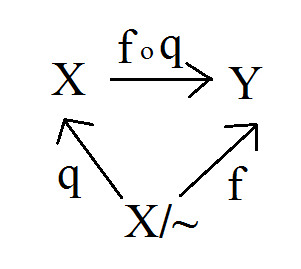
\includegraphics[width = 0.25\linewidth]{19_1.png}}
	\end{figure}
	\textbf{Теорема 2}:(универсальное свойство факторпространства)\\
	Пусть $Y$ -- топологическое пространство, $f:\ X\Rightarrow Y$ непрерывно постоянно на классах эквивалентности(то есть если $x_1 \sim x_2 \Rightarrow f(x_1) = f(x_2))$. Тогда $\exists$ единственное $\overset{\sim}{f}:\ X\slash \sim\ \Rightarrow Y$, делающее эту диаграмму коммутативной, и оно непрерывно.\\
	\textbf{Доказательство}: $\forall U\in X\slash \sim$ выберем $x\in U$, положим $\overset{\sim}{f}(U)=f(x)$. Если $x_1, x_2 \in U \Rightarrow x_1 \sim x_2 \Rightarrow f(x_1) = f(x_2) \Rightarrow \overset{\sim}{f}$ -- корректно определено. По построению диаграмма коммутативна и $\overset{\sim}{f}$ -единственное отображение, делающее ее коммутативно. Непрерывность $\overset{\sim}{f}$ -- из теоремы (1).\\
	\begin{figure}[h]
		\center{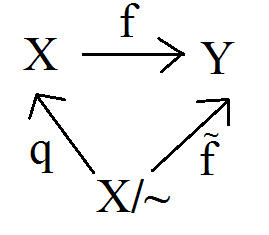
\includegraphics[width = 0.25\linewidth]{19_2.png}}
	\end{figure}
	\textbf{Определение}: $X, Y$ -- топологическое пространства. Отобрадение $f:\ X \Rightarrow Y$ -- факторное $\Leftrightarrow f$ сюръективно, и топология на $Y$ -- фактортопология, порожденная $f$. Иначе говоря: $U\subset Y$ -- открытое $\Leftrightarrow f^{-1}(U)$ открыто в $X$.\\
	\textbf{Теорема 3}: X, Y-топологическое  пространства. $f: X \Rightarrow Y$ факторное. Введем отношение эквивалентности на $X: x_1 \sim x_2 \Leftrightarrow f(x_1) = f(x_2)$. Тогда $\exists$ единственный гомеоморфизм $\overset{\sim}{f} : X\slash \sim \Rightarrow Y$, делающий диаграмму коммутативной.
	\textbf{Доказательство}: Теорема 2 $\Rightarrow \exists$ единственное непрерывное $\overset{\sim}{f}$ делающее диаграмму комутативной. $\overset{\sim}{f}(X\slash \sim)=\overset{\sim}{f}(q(x)) \Rightarrow f(x) = Y \Rightarrow \overset{\sim}{f}$-сюръекция. Пусть $\overset{\sim}{f}(U)=f(x)$, $\overset{\sim}{f}(V) = f(y) \Rightarrow f(x) =f(y) \Rightarrow x\sim y \Rightarrow U=V \Rightarrow \overset{\sim}{f}$-инъекция. Пусть $U\subset X\slash \sim$ открыто и $f^{-1}(\overset{\sim}{f}\setminus U)=q^{-1}(U)$ из компактности диаграммы и биективности $\overset{\sim}{f}. q^{-1}(U)$ открыто в $X: f$-факторное $\Rightarrow \overset{\sim}{f}(U)$-открыто в $Y \Rightarrow \overset{\sim}{f}$ открыто $\Rightarrow \overset{\sim}{f}$-гомеоморфизм.\\
	\begin{figure}[h!]
		\centering
		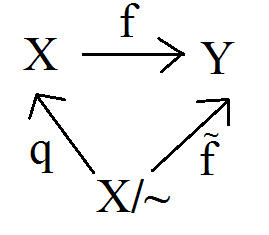
\includegraphics[width = 0.25\linewidth]{19_2.png}
	\end{figure}\\
	\textbf{Определение}: $X,Y$ -- множества, $f:\ X \Rightarrow Y$ -- сюръекция. Насыщение подмножества $A\subset X$ (относительно $f$) -- множество $f^{-1}(f(A))\subset X$. $A$ насыщенно $\Rightarrow A = f^{-1}(f(A))$\\
	\textbf{Теорема 4}: $X,Y$ -- множества, $f:\ X \Rightarrow Y$ -- непрерывная сюръекция. Следующие 3 свойства эквивалентны:\\
	\begin{enumerate}
		\item 
		$f$ -- факторное
		\item 
		$\forall $ насыщенного открытого $U \subset X f(U)$ открыто в $Y$
		\item 
		$\forall $ насыщенного замкнутого $B \subset X f(B)$ замкнуто в $Y$
	\end{enumerate}
	\textbf{Доказательство}:\\
	$(1) \Rightarrow (2)$ Пусть $U\subset X$ -- открытое насыщенное. $f^{-1}(f(U)) = U$ -- открыто, $f$ -- факторное $\Rightarrow f(U)$ -- открытое \\
	$(2) \Rightarrow (1)$ Пусть $V\subset Y$ таково, что $f^{-1}(V)$ открыто и насыщенно $\Rightarrow f^{-1}(f(V))$ -- открыто в $Y, f$ -- сюръекция $\Rightarrow V=f^{-1}(f(V)) \Rightarrow V$ -- открыто\\
	$(1)\Leftrightarrow (3)$ -- аналог. (1)$\Leftrightarrow$(2)\\
	Следствия: 
	\begin{enumerate}
		\item 
		$f:\ X\Rightarrow Y$ непрерывное сюръективное отображение. Если $f$ открыто или замкнуто, то $f$ -- факторное
		\item 
		$X$ -- компактное топологическое пространство, $Y$ -- хаусдорфово топологическое пространство. $f:\ X\Rightarrow Y$ непрерывное сюръективное отображение $\Rightarrow f$ -- факторное
		\item 
		$f:\ X\Rightarrow Y\ \text{факторное,}\ Z \subset X$ насыщенно и либо открыто, либо замкнуто $\Rightarrow f|_{Z}: z \Rightarrow f(z)$ -- факторное 
	\end{enumerate}


\newpage
%-----------------------------------------------------------------------------
\section{}
	\textbf{Частные случаи факторизации: стягивание подмножества в точку и склейка по отображению. Примеры. Вещественное проективное пространство, его эквивалентные определения (как факторпространство $\mathbb{R}^{n+1} \backslash \{0\}$ и как факторпространство $S^n$), компактность и хаусдорфовость.}\\
	\\
	$X$ -- топологическое пространство, $A \subset X$. Введем отношение эквивалентности на $X:\ x\sim y \Leftrightarrow$ либо $x = y$, либо $x, y \in A$. $X\slash A = X\slash \sim$, говорят: $X\slash A$ получено из $X$ стягиваением $A$ в точку.\\
	\textbf{Пример} $[0,1]\slash\{0;1\} \cong S^1$\\
	\textbf{Пример} $D=\{(x,y)\in \mathbb{R}^2:\ x^2+y^2=1\}\\
	\overline{D}=\{(x,y)\in \mathbb{R}^2:\ x^2 + y^2 \leqslant 1\}$\\
	Покажем, что $\overline{D}\slash S^1 \cong S^2$\\
	$S^2=\{(x,y)\in \mathbb{R}^3:\ x^2 + y^2 +z^2=1\}$\\
	Зафиксируем гомеофорфизм $h_1:\ D \Rightarrow \mathbb{R}^2$ и $h_2:\ {(\mathbb{R}^2)}_{+} \Rightarrow S^2$. Из свойств одноточечной компактификации $\Rightarrow \exists$ отображение $f:\ \overline{D} \Rightarrow S^2$, такое что диаграмма коммутативна и $f(p) = N\ \forall p \in S^1$, где $N=h_2(\infty).\ f$ непрерывно, сюръективно, $u \sim v \Leftrightarrow f(u) = f(v) \Rightarrow$ (по след.2) $f$-факторное $\Rightarrow S^2 \cong \overline{D}\slash S^1$\\
	\begin{figure}[h]
		\center{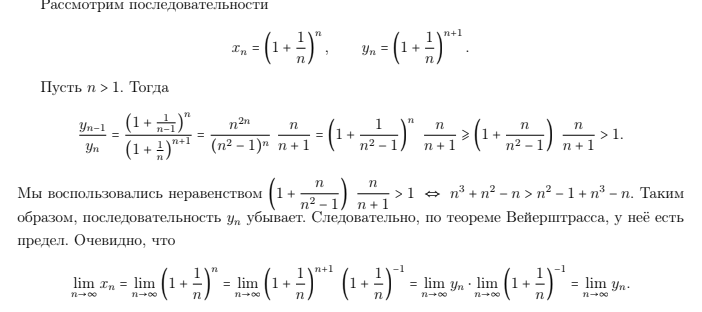
\includegraphics[width = 0.25\linewidth]{20_1.png}}
	\end{figure}
	$X,Y$ -- топологическое  пространства, $A\subset Y.\ f:\ A \Rightarrow X$ непрерывно. Введем отношение эквивалентности на $X \bigsqcup Y:\ \forall a\sim f(a)$, остальные классы -- одноэлементные множества. \\
	Обозначение $X {\cup}_{f} Y=(X \bigsqcup Y)\slash \sim$ -- склейка на $X$ и $Y$ по $f$.\\
	\textbf{Пример} $f = i_{S^1)}: S^1 = \partial \overline{D}\Rightarrow \overline{D}$ -- отображение включения. Покажем, что $\overline{D} {\cup}_{f} \overline{D} \cong S^2$.
	Обозначим: $\overline{D}_{+} = \overline{D}_{-} = \overline{D}$. Рассмотрим $g: \overline{D}_{+}\bigsqcup \overline{D}_{-}=\overline{D}$.\\
	$g(x,y)= 
	\begin{cases}
	(x,y,\sqrt{1 - x^2 - y^2)}\ \text{если}\ (x,y)\in \overline{D}_{+}\\ 
	(x,y, -\sqrt{1 - x^2 - y^2)}\ \text{если}\ (x,y)\in \overline{D}_{-}
	\end{cases}$
	$g$ непрерывно, сюръективно $\Rightarrow$ по следствию (2): $p\sim q \Leftrightarrow g(p) = g(q) \Rightarrow \overline{D} {\cup}_{f} \overline{D} \cong S^2.$
	\begin{figure}[h]
		\center{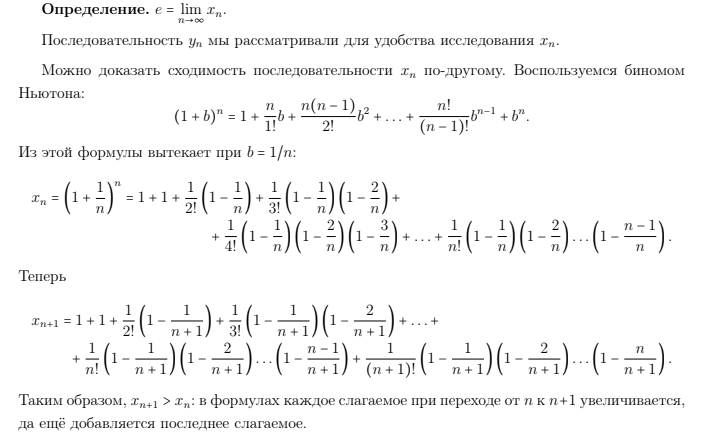
\includegraphics[width = 0.25\linewidth]{20_2.png}}
	\end{figure}
	\textbf{Пример} ВЕЩ. ПРОЕКТИВНОЕ ПРОСТРАНСТВО\\
	$\mathbb{R} \mathbb{P}^n \cong S^n\slash\sim$, где $x\sim y \Leftrightarrow x = y$, либо $x = -y$ (здесь $S^n=\{x = x_0,\ldots ,x_n\}\in \mathbb{R}^{n + 1}:\ \sum\limits^{n}_{i = 0} x_i^2=1$)\\
	\textbf{Доказательство}: $q_1, q_2$ -- отображения факторизации.
	\begin{figure}[h]
		\center{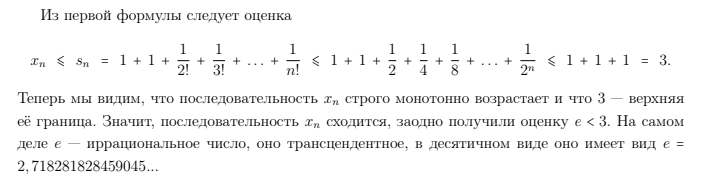
\includegraphics[width = 0.25\linewidth]{20_3.png}}
	\end{figure}
	$\Rightarrow \exists$ единственное непрерывное $f$ такое, что диаграмма коммутативна, $f$ -- биекция( по построению). Рассмотрим $\rho: \mathbb{R}^{n + 1}\slash\{0\} \Rightarrow S^n,\ \rho(v) = \frac{v}{||v||} \Rightarrow \exists$ единственное непрерывное $g$ такое, что диаграмма коммутативна $\rho \circ i_{S^n} = id_{S^n} \Rightarrow g \circ f=\text{id}_{S^n}\slash\sim \Rightarrow g=f^{-1} \Rightarrow f^{-1}$ - непрерывно $\Rightarrow f$ -- гомеоморфно\\
	\textbf{Следствие}: $\mathbb{R} \mathbb{P}^n$ компактно и хасудорфово.\\
	\textbf{Доказательство}: Пусть $x,y \in S^n,\ x\nsim y\Rightarrow x,y, -x, -y$ попарно различны $\Rightarrow \exists r\textgreater 0$ такое, что $B_r(x), B_r(y), B_r(-x), B_r(-y)$ попарно не пересекаются. Обозначим $U=B_r(x)\cup B_r( - x),\ V = B_r(y)\cup B_r(-y) \Rightarrow S^n\cap U$ и $S^n\cap V$ открыты, насыщенны и не пересекаются, $x\in S^n\cap U, y\in S^n\cap V \Rightarrow S^n\slash \sim$ хаусдорфово\\
	\begin{figure}[h]
		\center{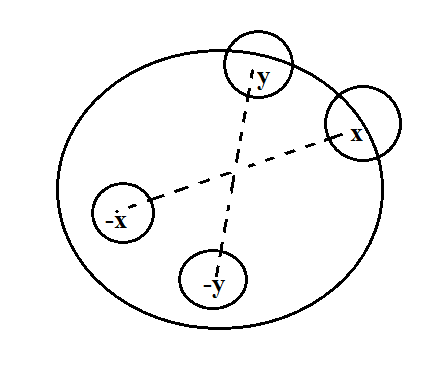
\includegraphics[width = 0.25\linewidth]{20_4.png}}
	\end{figure}

\newpage
%-----------------------------------------------------------------------------
\section{}
	\textbf{Регулярные и нормальные топологические пространства. Характеризации регулярности и нормальности в терминах окрестностей. Регулярность локально компактных хаусдорфовых пространств. Нормальность компактных хаусдорфовых пространств и метризуемых пространств.}\\
	\\
	\textbf{Определение}: топологическое пространство $X$ называется:\\
	\begin{enumerate}
		\item 
		регулярным $\Leftrightarrow$ оно удовлетворяет $T_1$ (точки замкнуты) и $\forall x\in X$ для любого замкнутого $B \subset X$, такое что $x$ не принадлежит $B$, существует открытые $U(x\in U),V (B\subset V)$, такие что $U\cap V=\varnothing$
		\item 
		нормальным $\Leftrightarrow$ оно удовлетворяет $T_1$ и для любых замкнутых $A, B$, такие что $A \cap B=\varnothing$, существуют открытые $U, V\subset X, A\subset U, B\subset V$ и $U\cap V=\varnothing$
	\end{enumerate}
	Наблюдение: нормальное $\Rightarrow$ регулярное $\Rightarrow$ хаусдорфово\\
	\textbf{Предположение} $X$ -- топологическое  пространство, удовлетворяющее $T_1$\\
	\begin{enumerate}
		\item 
		$X$ регулярное $\Leftrightarrow \forall x\in X$ для любого открытого $W\ (x\in W)$ существует открытое $U$, такое что $x\in U, \overline{U} \subset W$
		\item 
		$X$ нормальное $\Leftrightarrow$ для любого замкнутого $A\subset X$ для любого открытого $W\supset A$ существует открытое $U$, такое что $A\subset U,\ \overline{U}\subset W$
	\end{enumerate}
	\textbf{Доказательство}: \\
	(2) Обозначим $W=X\slash B$, где $B$-из определения нормированного пространства\\
	$X$ нормальное $\Leftrightarrow$ для любого замкнутого $A \subset X$, для любого открытого $W\subset X$, такое что $A\subset W$, существует открытое $U\supset A$, и существует замкнутое $C\subset W$(здесь $C=x\slash V, V$-из опредления нормированного пространства), такое что $U\subset C \Leftrightarrow$ для любого замкнутого $A\subset X$, для любого открытого $W\supset A$, существует открытое $U \supset A$, такео что $\overline{U}\subset W$ что и требовалось доказать\\
	(1) аналогично\\
	\\
	\textbf{Предположение}: Локально компактное хаусдорфово пространство регулярно\\
	\textbf{Доказательство}: ранее доказанное свойство из п.1 предыдущего предложения\\
	\\
	\textbf{Предположение} 
	\begin{enumerate}
		\item 
		компактно хасудорфово пространство нормально
		\item 
		метризуемое пространство нормально
	\end{enumerate}
	\textbf{Доказательство}: казалось бы, это упражнение, но нет, доказательство будет позже\\
	\textbf{Обозначение}: $(X, \rho)$ -- метрическое, $A\subset X, x\in X\\
	\rho(x, A)=\text{inf}\{\rho(x,a): a\in A\}$-расстояние от $x$ до $A$\\
	\textbf{Лемма}: \\
	\begin{enumerate}
		\item 
		$\rho(x, A)=0 \Leftrightarrow x\in \overline{A}$
		\item 
		функция $x \Rightarrow \rho(x, A)$ на $X$, 1 -- липшицево (и поэтому непрерывна)
	\end{enumerate}
	\textbf{Доказательство}: \\
	(1)-почти очевидно \\
	(2)$\forall x,y \in X \forall a\in A \rho(x,a) \leqslant \rho(x,y)+ \rho(y,a)$. Берем $text{inf}(a\in A) \Rightarrow \rho(x, A) \leqslant \rho(x,y) + \rho(y, A) \Rightarrow \rho(x, A)-\rho(y, A) \leqslant \rho(x,y) \Leftrightarrow \rho(y, A)- \rho(x, A) \leqslant \rho(x,y) \Rightarrow |\rho(x, A)- \rho(y, A)| \leqslant \rho(x,y)$ что и требовалось доказать\\
	\\
	Доказательство предложения, которое было выше: \\
	(1)$A, B \subset X$ замкнуты, $A\cap B= \varnothing$. $X$ -- компактно $\Rightarrow A, B$ компактно\\
	Знаем, $\forall x\in A \exists$ открытые $U_x, V_x$, такие что $x\in U_x, B \subset V_x, U_x \cap V_x=\varnothing$\\
	$\exists x_1, \ldots , x_n \in A$, такое что $A \subset \overset{n}{\underset{i = 1}{\cup}} U_{x_i}$\\
	$U, V$ открытые, $A \subset U,\ B \subset V,\ U\cap V=\varnothing$ \\
	(2) $A,B \subset X$ замкнуто, $A\cap B=\varnothing$ \\
	Рассмотрим $f(x)=\frac{\rho(x,A)}{\rho(x, A)+ \rho(x, B)}$. Из Леммы: $f$ непрерывно, $f_{|A}=0, f_{|B}=1, f:\ X \Rightarrow [0,1]$\\
	Обозначим: $U=f^{-1} ([0, \frac{1}{2})), V=f^{-1} ((\frac{1}{2}, 1])$\\
	$U, V$ открыты, $U \supset A,\ V \supset B,\ U\cap V=\varnothing$ что и требовалось доказать\\
	

\newpage
%-----------------------------------------------------------------------------
\section{}
	\textbf{Лемма Урысона.}\\
	\\
	\textbf{Лемма Урысона}: $X$ -- нормальное топологическое пространство, $A, B \subset X$ замкнуто, $A\cap B=\varnothing$. Тогда для любого отрезка $[a,b] \subset \mathbb{R}$ существует непрерывное $f: X \Rightarrow [a,b]$, такое что $f_{|A} = a,\ f_{|B}=b$\\
	\textbf{Доказательство}: можем считать: $[a,b]=[0,1]$\\
	Обозначим: $U_1=X\slash B$. Тогда $A\subset U_1$\\
	Существует открытое $U_{\frac{1}{2}}$, такое что $A\subset U_{\frac{1}{2}} \subset \overline{U_{\frac{1}{2}}} \subset U_1$\\
	Существуют открытые $U_{\frac{1}{4}},\ U_{\frac{3}{4}}$ такие что $A\subset U_{\frac{1}{4}} \subset \overline{U_{\frac{1}{4}}} \subset U_{\frac{1}{2}} \subset \overline{U_{\frac{1}{2}}} \subset U_{\frac{3}{4}} \subset \overline{U_{\frac{3}{4}}} \subset U_1$ и тд\\
	Обозначим: $D = \{r\in [0,1]:\ r\ \text{-- двоичное рациональное}\} = \{\frac{k}{2^n},\ n\in \mathbb{N},\ k=1,\ldots,2^n\}$\\
	$D$ плотно на $[0,1]$\\
	По индукции: $\forall r \in D$ построим открытое $U_r \subset X$, такое что $\forall x,\ s\in D,\ r\textless s$, выполняется: $A\subset U_r \subset \overline{U_r} \subset U_s \subset \overline{U_s} \subset U_1 (*)$\\
	Рассмотрим $f:\ X \Rightarrow [0,1],\ 
	f(x)=
	\begin{cases}
	1,\ x\in B \\
	\text{inf} \{r\in D:\ x\in U_r\},\ x\ \text{не принадлежит}\ B
	\end{cases}\\
	f_{|A}=0,\ f_{|B} = 1$ по построению. Осталось доказать непрерывность $f$\\
	Достаточно доказать $\forall t\in (0,1)\ f^{-1} ([0,t))$ и $f^{-1}((t, 1])$ открыты в $X$\\
	$f(x) \textless t \Leftrightarrow \exists r \in D$, такое что $r\textless t$ и $x\in U_r$\\
	Поэтому: $f^{-1} ([0,t)) = \overset{}{\underset{r\textless t}{\cup}} U_r$ -- открыто\\
	$f(x) \textgreater t \Leftrightarrow \exists x\in D$, такое что $x\textgreater t$ и $x$ не принадлежит $\overline{U_r}$, то есть $x\in X\slash \overline{U_r}$\\
	Поэтому $f^{-1} ((t,1])=\overset{}{\underset{r \textgreater t}{\cup}} (X\slash U_r)$ что и требовалось доказать


\newpage
%-----------------------------------------------------------------------------
\section{}
	\textbf{Теорема Титце-Урысона.}\\
	\\
	\textbf{Теорема Титце - Урысона}: $X$-нормальное топологическое пространство, $Y\subset X$-замкнуто, $Z=[a,b] \subset \mathbb{R}$, либо $Z=\mathbb{R}^n$\\
	Тогда для любого непрерывного $f: Y \Rightarrow Z$ существует $g: X \Rightarrow Z$, такое что $g_{|Y}=f$\\
	\\
	\textbf{Лемма 1}: $X$-нормальное топологическое пространство, $Y\subset X$ замкнуто, $f: Y \Rightarrow [ - a,a]$ непрерывно ($a\textgreater 0) \Rightarrow$ существует непрерывное $g: X \Rightarrow [ - \frac{a}{3}, \frac{a}{3}]$, такое что $\forall y\in Y |f(y) - g(y)| \leqslant \frac{2a}{3}$\\
	\textbf{Доказательство}: обозначим $A=f^{-1} ([ - a,- \frac{a}{3}]), B=F^{-1} ([\frac{a}{3}, a]). A,B$ замкнуты, $A\cap B=\varnothing$. По \textbf{Лемме Урысона}: $\exists g: X \Rightarrow [ - \frac{a}{3}, \frac{a}{3}]$, такое что $g_{|A}= - \frac{a}{3}, g_{|B}=\frac{a}{3} \Rightarrow g$ -- искомая\\
	\\
	\textbf{Лемма 2}: $X$-банахово пространство( то есть полное нормированное пространство). $x_1,x_2,\ldots \in X$. Предположим $\overset{\infty}{\underset{n = 1}{\sum}} ||x_n|| \textless \infty \Rightarrow$ ряд $\sum x_n$ сходится в $X$ (то есть $\exists \lim_{n\rightarrow \infty} \overset{n}{\underset{k = 1}{\sum}} x_n \in X)$ к некоторому $x\in X$, и $||x|| \textless \sum ||x_n||$\\
	\textbf{Доказательство}: как для $\mathbb{R}$\\
	\\
	\textbf{Доказательство ТЕОРЕМЫ}: \\
	\textbf{Случай 1}: $Z=[a,b]$. Можем считать, $z=[ - 1,1]$\\
	По Лемме 1: существует непрерывное $g: X \Rightarrow [ - \frac{1}{3}, \frac{1}{3}]$, такое что $\forall y\in Y |f(y)- g_0 (y)| \textless \frac{2}{3}$\\
	По Лемме 1: существует непрерывно $g_1: X \Rightarrow [ - \frac{1}{3}\cdot \frac{2}{3}, \frac{1}{3}\cdot \frac{2}{3}]$, такое что $\forall y\in Y |f(y)- g_0 (y)-g_1 (y)| \textless {\frac{2}{3}}^2$ и тд\\
	Лемма 1+индукция: $\forall n\in \mathbb{N}$, существует $g_n: X \Rightarrow [ - \frac{1}{3}\cdot {\frac{2}{3}}^n, \frac{1}{3}\cdot {\frac{2}{3}}^n]$, такое что $\forall y\in Y |f(y)- \sum g_k (y)| \textless {\frac{2}{3}}^n (*)$\\
	$(C_b(X), ||\cdot||_{\infty})$-банахово пространство\\
	$g_n\in C_b(X), ||g_n||_{\infty} \leqslant \frac{1}{3} \cdot ({\frac{2}{3}})^n$\\
	По Лемме 2: $\exists g=\overset{\infty}{\underset{n = 0}{\sum}} g_n \in C_b (X), ||g||_{\infty} \leqslant \frac{1}{3} \overset{\infty}{\underset{n = 1}{\sum}} (\frac{2}{3})^n=1$\\
	При $n\to \infty$ из $(*)$ получаем: $|f(y) - g(y)|=0\ \forall y \in Y$, то есть $g_{|Y} = f$\\
	\\
	\textbf{Случай 2}: $Z=\mathbb{R}$. Можем считать, что $Z=( - 1,1)$ (так как $( - 1,1)$ и $\mathbb{R}$ гомеоморфны)\\
	Из случая 1 следует, что существует непрерывное $h: X \Rightarrow [0,1]$, такое что $h_{|Y}=1, h_{|B}=0$\\
	Обозначим: $g=h \phi \Rightarrow g$ непрерывно, $g_{|Y}=f, g(X) \subset ( - 1,1) \Rightarrow g$-искомая\\
	\\
	\textbf{Случай 3}: $Z=\mathbb{R}^n\\
	f=(f_1, \ldots , f_n): Y\Rightarrow \mathbb{R}^n, f_i : Y \Rightarrow \mathbb{R} \forall i= 1,\ldots , n$\\
	К каждому $f$ применим случай 2 и получим искомое $g=(g_1,\ldots ,g_n): X\Rightarrow \mathbb{R}^n $

